\documentclass{article}[gray]
\usepackage[utf8]{inputenc}
\usepackage{tikz}
\usepackage{pgfplots}
\usepackage{amsmath}
\usepackage{geometry}
\geometry{a5paper, margin = 0.5in, footskip = 0.255in}
\numberwithin{equation}{subsection}
\usepackage{textcomp}
\usepackage{rotating}
\usepackage{esint}
\pgfplotsset{width=10cm,compat=1.9}
\setlength{\parindent}{1cm}
\renewcommand{\baselinestretch}{1.5}

\begin{document}

\begin{center}
\
\newline
\newline
\newline
\newline
\newline
\newline
\newline
\newline
\newline
\newline
\newline

\textbf{\LARGE Leo's Guide to AP Physics C: Mechanics}
\end{center}
\begin{center}
Copyright \textcopyright \ 2019 by Leonardo Bonanno
\end{center}
\begin{center}
\footnotesize ISBN 9781729432624


\end{center}
\newpage
\tableofcontents
\newpage

\section{Forward}
Hello. My name is Leonardo Bonanno. As of this writing, I am a high-school student at Gulliver Preparatory School in Miami, Florida. When I was in 9th grade, I wanted to learn about physics. However, I found myself bored with thoughtless problems that did not help when I had to solve difficult problems. Anyone can plug in numbers into equations, but understanding these equations is much more difficult and much more powerful. So, throughout this book, I hope to equip you with the tools to not only do well on the AP Physics C exam but to understand the tools of elementary physics and the beauty of the subjects. Thank you, and I hope you enjoy this book.
\newline
-Leo

\pagebreak

\section{Kinematics}

\subsection{Instantaneous Velocity and Some Philosophy}

Instantaneous velocity is one of the simplest concepts in physics, but it is rather odd when you think about it more deeply. How can something be moving at a given moment? If it is stuck in a moment, how can it have any velocity? Isn't the instantaneous velocity at any moment in time just 0 as an object can't be in two places at one time? These are all philosophical questions I had when starting physics that were not quite addressed but that I came just to ignore. It is of little help to philosophize in these ways and, unfortunately, these lines of reasoning will not help us find anything useful. Even though philosophizing about physics is quite interesting, it is not particularly relevant for doing physics. Like Feynman and others have said, at many levels, we only understand the world at the level of the equations. The simple truth is that things can have a velocity at a given moment, and the velocity can be changing over time, but at any given moment it is fixed.
\vspace{5mm}
\\
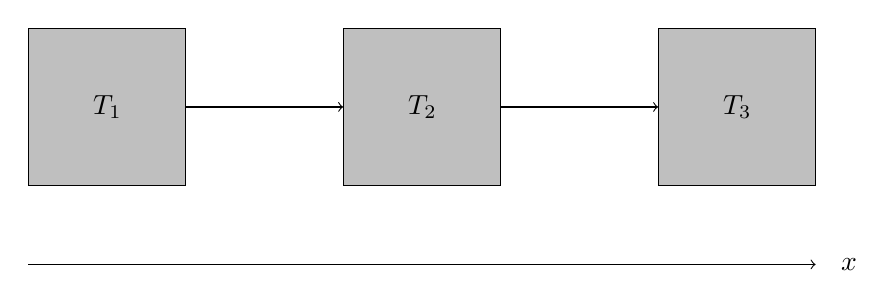
\begin{tikzpicture}
\filldraw[color = black, fill = lightgray] (0,0) rectangle (2,2);
\draw[black] (0.7,1) node[anchor=west] {$T_1$};
\draw[->] (2,1) -- (4,1);
\filldraw[color = black, fill = lightgray] (4,0) rectangle (6,2);
\draw[black] (4.7,1) node[anchor=west] {$T_2$};
\draw[->] (6,1) -- (8,1);
\filldraw[color = black, fill = lightgray] (8,0) rectangle (10,2);
\draw[black] (8.7,1) node[anchor=west] {$T_3$};
\draw[->] (0,-1) -- (10,-1);
\draw[black] (10.2,-1) node[anchor=west] {$x$};
\end{tikzpicture}
\newline
Defining the position as $x$ and assuming the motion is only in one definition, we can define the instantaneous velocity as
\begin{equation} \label{eq:a}
v\left(t\right) = \frac{dx}{dt}\end{equation}

 at the moment $t$. With this definition, we are going to think of instantaneous velocity as the limit of the average velocity as the interval over which we are averaging goes to zero.  However, even though instantaneous velocity is defined in the way it is, I like to think about it a different way. $$
v\left(t\right) = f\left(t\right)$$ for some velocity function $f\left(t\right)$. When we represent velocity in this way, we are thinking about velocity as a function of the force that is being imparted onto an object(which subsequently relies on time, thus we write $\left(t\right)$. We instead can think about instantaneous velocity as the velocity a particle would stay at if all forces acting on an object were suddenly removed at a given time. So when we have a constant force such as gravity imparting a force on an object, the instantaneous velocity will be the velocity of the object if that force were taken away. This may seem rather odd, but it can help elucidate some of our ideas of velocity and connect them to Newtonian dynamics which we will study soon. This is useful because velocity is fundamentally linked to the different forces on an object as we will see with Newton's laws. 

\subsection{Velocity and Speed}
\vspace{5mm}
\begin{tikzpicture}
\draw[circle] (0,0) circle (0.0001cm);
\draw[->] (4,0) -- (8,2);
\draw[black] (6,-0.5) node[anchor = west] {$V_x$};
\draw[black] (6,-0.5) node[anchor = west] {$V_x$};
\draw[dashed] (4,0) -- (8,0);
\draw[dashed] (8,0) -- (8,2);
\draw[black] (8.125,1) node[anchor = west] {$V_y$};
\draw[black] (5.75,1.5) node[anchor = west] {\begin{turn}{45} $\vec{V}$ \end{turn}};
\end{tikzpicture}
\newline
The first topic that you learn about when you begin studying physics is kinematics. Velocity is simply the derivative of position with respect to time. Quite frankly, I do not like the definition being given in this way. Velocity is a measure of how the position of something is changing over time. Normally, this something is just an object, but it does not necessarily have to be. For example, the center of mass of a system can have a velocity as well. We will see this later. As a reminder, our precise formula for velocity is $ \vec{v}= \frac{d\vec{r}}{dt}$. Where $\vec{r}$ is the position of our "thing." We assume that $\vec{r}$ is a position vector. We can normally assume that if a problem deals with the position of something changing over time, the original position of the thing should be defined as the origin. This is usually very convenient. Velocity, after position, is the second physical quantity that is seen as a vector in the standard physics curriculum. It is important to understand that we can view velocity in general as a vector of the form \begin{equation} \vec{v}= <x,y,z>\end{equation} Where $|\vec{v}|$ is the magnitude of the velocity and \begin{equation}\frac{\vec{v}}{|\vec{v}|}\end{equation} is the direction of the velocity. In some sense, we can think of the components of the velocity as not impacting each other. We can think of them as being in some sense independent. By this I mean, if a force is imparted onto an object that changes its velocity. The change in velocity in each direction is only impacted by force imparted in that direction. This will prove very relevant when we begin studying free fall and the throwing of objects. Now that we have defined velocity, we can define speed. Speed is simply the magnitude of the velocity vector. If you are given the speed of an object and direction of this speed, you can find the velocity vector of the object. This is simple enough when the speed is constant; however, in practice, the speed is changing, so if we want to think about the actual path of the object, it is usually easier to work with velocity than with speed. In fact, velocity is used far more often than speed and speed is the only common scalar that we will encounter in kinematics. Once we start studying acceleration and jerk, we will see that the magnitudes of these vectors, unlike speed, are simply called “the magnitude of XXX." 
\clearpage
\subsection{Acceleration and Constant Acceleration Motion}
%Car I
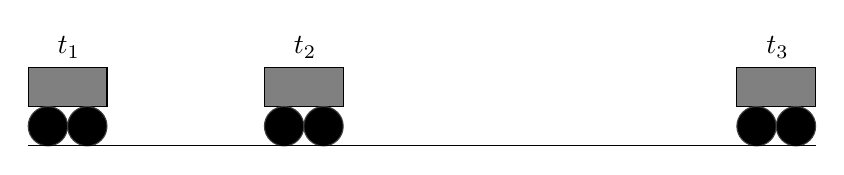
\begin{tikzpicture}
\filldraw[draw = black, fill = gray] (0,0) rectangle (1,0.5);
\filldraw[fill = black, draw = darkgray] (0.25,-0.25) circle (0.25cm);
\filldraw[fill = black, draw = darkgray] (0.75,-0.25) circle (0.25cm);
%Car II
\filldraw[draw = black, fill = gray] (3,0) rectangle (4,0.5);
\filldraw[fill = black, draw = darkgray] (3.25,-0.25) circle (0.25cm);
\filldraw[fill = black, draw = darkgray] (3.75,-0.25) circle (0.25cm);
%Car III
\filldraw[draw = black, fill = gray] (9,0) rectangle (10,0.5);
\filldraw[fill = black, draw = darkgray] (9.25,-0.25) circle (0.25cm);
\filldraw[fill = black, draw = darkgray] (9.75,-0.25) circle (0.25cm);
\draw[black] (0,-0.5) -- (10,-0.5);
\draw[black] (0.25,0.75) node[anchor=west] {$t_1$};
\draw[black] (3.25,0.75) node[anchor=west] {$t_2$};
\draw[black] (9.25,0.75) node[anchor=west] {$t_3$};
\end{tikzpicture}

Acceleration is significant in kinematics and dynamics, particularly 
because of Newton's Laws. From a strictly kinematic perspective, we can interpret Newton’s Laws as saying that a force(which we will not define for now) causes a body to have an acceleration that is a function of time. This is often presented as nothing more than a truth of nature, but it is important to understand that forces do not cause a body to have constant velocity but rather constant acceleration. While this might seem trivial, problems involving this idea are rife in elementary physics. For now, let us define linear acceleration(as opposed to angular or centripetal acceleration; which we will define later). Acceleration is defined as the rate of change of the velocity of an object with respect to time. Before introducing instantaneous acceleration, first, we have to introduce average velocity. Average acceleration is simply the change in velocity for a given time period divided by the length of the small time period. \begin{equation} = \frac{1}{t_2-t_1} \int_{v_1}^{v_2} dv\end{equation} From this definition of average acceleration it is natural to see why we would want to define an instantaneous acceleration just like we wanted to define an instantaneous velocity. This definition begs the question, "What happens as $t_2-t_1$ goes to 0. When we take the limit, we find that instantaneous acceleration can be defined as $$\frac{d\vec{v}}{dt}$$ or as $$\frac{d^2\vec{x}}{dt^2}$$ These two expressions; however, are exactly the same because $$\vec{v}= \frac{d\vec{x}}{dt}$$ so $$\frac{d\vec{v}}{dt} = \frac{d}{dt}\left(\frac{d\vec{x}}{dt}\right) = \frac{d^2\vec{x}}{dt^2}$$ Integrating our definition of velocity over time we find that $\vec{v} = \int \vec{a} \ dt$. While of course in the general case of acceleration, acceleration is changing as a function of time, for most of the problems we will see, acceleration is assumed to be constant. Frankly, we often assume this because if we have a changing acceleration, then the math can get much hairier when dealing with dynamics problems. To give a preview of the future, trying to solve dynamics problems using Newton's first law $\vec{F}=m\vec{a}$ can get quite odd when assuming acceleration to be changing because both the force and acceleration vectors are changing as functions of time. This forces us to use methods of differential equations which is beyond the scope of this book. Now, we can start thinking about motion with constant acceleration. When discussing this topic, there are often a few great formulas that are introduced to solve these types of problems. They are important, but please do not memorize them. They can all be learned and derived from first principles. The first introduction equation is pretty simple \begin{equation} v=v_o+at\end{equation} This equation is saying that the velocity of the object at hand started at a certain fixed velocity and is increasing by a factor of $a$ with time, where $a$ is the velocity of the object. It is important to recognize that often the initial velocity will not be given directly. Instead, the problem will state that a change in velocity has occured over a certain time period. The question may ask for the time period of the velocity change? Here we can write $\Delta v= at$. The second equation is perhaps more hairy, \begin{equation}x = x_0 + v_0 t+\frac{1}{2}at^2\end{equation} If you have already seen Taylor series you can probably guess what the next term would be if the acceleration were changing at a constant rate. The Taylor series is ultimately where this comes from, but we do not need to worry about this here. This equation can be simply derived from the following fact $\vec{x}= \vec{x_0} + \int \vec{v} dt$.  If we have from equation 1 that $v = v_o+at$ we can integrate this with respect to time to find \begin{equation}\Delta x = v_ot+\frac{1}{2}at^2\end{equation} But $\Delta x = x-x_0$, so with rearrangement we arrive at our original equation. The final and perhaps most useful equation for the AP Exam is \begin{equation} v^2=v_0^2+2a \Delta x\end{equation} This comes in very handy when we are not given any information about the time period over which velocity has changed, and we want to find the distance traveled by the object. The derivation is straightforward and can be derived using the first and second equations and nothing else. This will be left as an exercise to the reader because it is important to understand this formula fully. Having formulas to solve constant acceleration problems will prove very useful when we begin problems in which the only force acting on a body is gravity. 
\newline
\newline
\begin{tikzpicture}
\draw (0,0) circle (0.0001cm);
\draw[black] (0,6.5) node[anchor = west] {Position vs Time Graph for Constant Acceleration Motion};
\draw[black] (-1,0) -- (-1,6);
\draw[black] (-1,0) -- (9,0);
\draw (-1,0) parabola (9,6);
\draw[black] (4,-0.5) node[anchor = west] {Time};
\draw[black] (-1.75,3) node[anchor = west] {\begin{turn}{90} Position \end{turn}};
\end{tikzpicture}
\newline
\subsection{Free Fall}
Freefall problems frequently occur in elementary physics examinations. These types questions normally follow a pretty standard format, as follows. First, a projectile has been launched from a certain angle at a certain velocity. Second, you will be asked to find something such as the total distance traveled by the projectile. The good thing about these problems is that once you understand them, they are simple. The difficult part of these problems is recognizing how the gravitational force only impacts a force in the vertical direction and that therefore the horizontal velocity of the projectile will remain constant throughout the flight of the projectile. I will not discuss them here as I find them to be more fun to solve on your own using the facts that I have been given. However, one other fact may prove useful. That is, at the peak of the flight of a projectile, the vertical velocity of the projectile must be 0. I urge you to think about this point for a little bit, and it should start to make sense. 
\newline
\newline
\newline
\newline
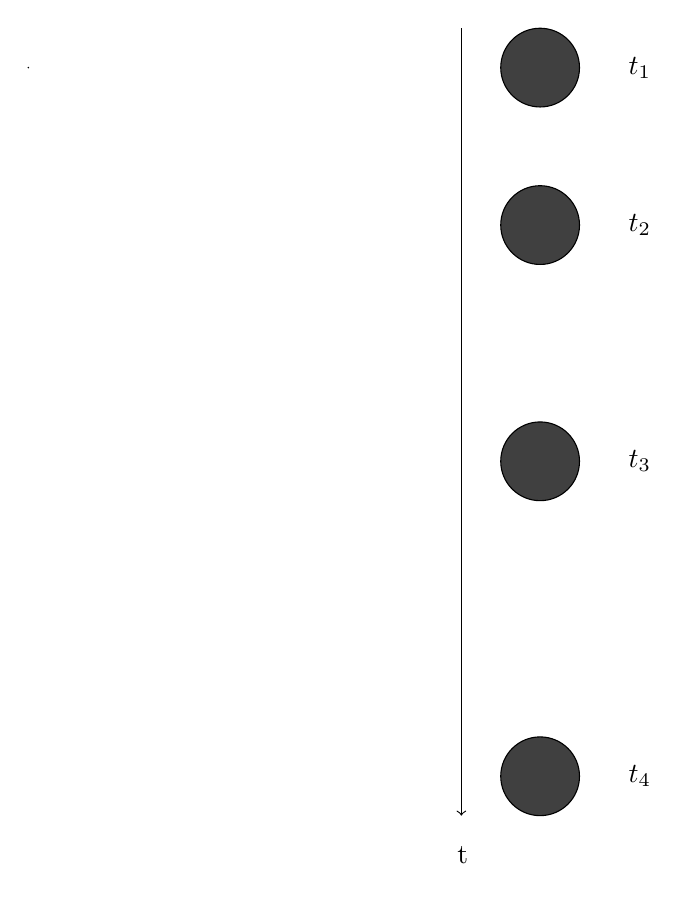
\begin{tikzpicture}
\filldraw[fill = darkgray, draw = black] (0,0) circle (0.001cm);
\filldraw[fill = darkgray, draw = black] (6.5,0) circle (0.5cm);
\filldraw[fill = darkgray, draw = black] (6.5,-2) circle (0.5cm);
\filldraw[fill = darkgray, draw = black] (6.5,-5) circle (0.5cm);
\filldraw[fill = darkgray, draw = black] (6.5,-9) circle (0.5cm);
\draw[->] (5.5,0.5) -- (5.5,-9.5);
\draw[black] (5.325,-10) node[anchor=west] {t};
\draw[black] (7.5,0) node[anchor=west] {$t_1$};
\draw[black] (7.5,-2) node[anchor=west] {$t_2$};
\draw[black] (7.5,-5) node[anchor=west] {$t_3$};
\draw[black] (7.5,-9) node[anchor=west] {$t_4$};
\end{tikzpicture}
\newline
\newline
\newline
\newline
\subsection{Jerk and The Calculus of Physics}
\begin{tikzpicture}
\begin{axis}[title = {Position vs. Time with Constant Jerk}, xlabel = {Time}, ylabel = {Position}, domain = 0:7]
\addplot[color=gray]{x^2/2+x^3/6};
\end{axis}
\end{tikzpicture}
\newline
The most natural question I had when learning elementary physics was, what happens kinematically and dynamically when the acceleration of an object we are examining is changing. The AP Physics Exam will only teach you about kinematics problems in which the acceleration is constant, but of course; in many real-world problems, the acceleration is changing. Sustaining constant acceleration requires quite a bit of energy especially when we consider the fact that friction exists. In order to work with non-constant acceleration problems, we can define \begin{equation}\vec{J}= \frac{d\vec{a}}{dt}\end{equation} where $\vec{J}$ is called jerk. Through the definitions of derivatives, we can show that jerk, while being equal to the first time-derivative of acceleration, is also equal to the second time derivative of velocity and the third time derivative of position. The most complex problem regarding the change of acceleration over time will be when we define the position of an object in linear space as a function $\vec{x}\left(t\right)$ where $\vec{x}\left(t\right)$ is a simple polynomial. Finding the velocity, acceleration, and jerk for this situation requires taking derivatives with respect to time. This is fairly simple and with enough practice will become a rote concept. I will not go over it more because it requires very little conceptual thinking. Perhaps more advanced is finding a velocity function for an object given an acceleration function $\vec{a}\left(t\right)$, and then finding a position  function using $\vec{v}\left(t\right)$. The important thing when doing these problems is to make sure we add a constant term to a function whenever we integrate over time. So in order to truly find a position function $\vec{v}\left(t\right)$ given an acceleration function $\vec{a}\left(t\right)$ we need to be given an initial value of $\vec{v}\left(t_0\right)$ at some  time $t_0$. This pair of $t_0$ and $\vec{v_0} \left(t\right)$ is called our initial condition. In differential equations, these initial conditions are critical. Quite frequently, we are told that initially, our body of interest is at rest. This is just another way of saying that our initial condition is given by $t_0=0$, $\vec{v_0}\left(0\right)=0$. So, for example, if we are given that a body is initially at rest and that $a\left(t\right)=t+1$. 

Note: In this example as in all others, the units will not match up as we assume that t is not 6 seconds but instead just 6 and $\vec{a}\left(t\right)$ is not 6 $\frac{m}{s^2}$ but rather only 6. However, when we use the acceleration as a function of time in an outside context, we must make sure to use the acceleration with the proper units as it can get quite confusing if we do not. 

We then have that \begin{equation}v\left(t\right)=6t+\frac{1}{2}t^2+C_1\end{equation} We can now plug in to find t. \begin{equation}6\left(0\right)+\frac{1}{2}\left(0\right)^2+C_1=0\end{equation} So $$C_1 = 0$$ and \begin{equation}v\left(t\right)=t+\frac{1}{2}t^2\end{equation} Next, we can try to find the change in position of the body as a function of time. If we are asked to find the change of a ball over time, this means we can assume that the ball is at position $\vec{x_0} = 0$ at time 0 because the change in position is 0 at time 0. So we now say that \begin{equation}x\left(t\right)=\frac{1}{2}t^2+\frac{1}{6}t^3+C_2\end{equation} However, we assumed that $x\left(0\right)=0$, so $0=0+0+C_2$. So $C_2=0$ and, finally, \begin{equation}x\left(t\right)=\frac{1}{2}t^2+\frac{1}{6}t^3\end{equation} Real world problems will not always be this trivial and sometimes the initial conditions will not be given conveniently at time and position being equal to 0. However, fundamentally, the concepts should work the exact same way when these conditions change.
\newline
\newline
\begin{tikzpicture}
\draw[dashed] (6,4) parabola (0,0) ;
\draw[dashed] (6,4) parabola (12,0);
\filldraw[color = black, fill = darkgray] (0,0) circle(0.25cm);
\filldraw[color = black, fill = darkgray] (6, 4) circle (0.25cm);
\filldraw[color = black, fill = darkgray] (12,0) circle(0.25cm);
\end{tikzpicture}
\clearpage
\section{Newton's Laws and Dynamics}

\subsection{What is a Force?}
\begin{tikzpicture}
\draw[black] (0,0) circle (0.001cm);
\filldraw[draw = black, fill = white] (5,0) rectangle (7,2);
\draw[->] (6,0) -- (6,-2);
\draw[black] (5.75,1) node[anchor = west] {M};
\draw[black] (5.75,-2.25) node[anchor = west] {$\vec{F_1}$};
\draw[->] (7,1) -- (9,1);
\draw[black] (9,1) node[anchor = west] {$\vec{F_2}$};
\draw[->] (5,1) -- (3,1);
\draw[black] (2.5,1) node[anchor = west] {$\vec{F_3}$};
\end{tikzpicture}

Before we even begin discussing Newton’s Laws, I think it is important to talk a little bit about what it also means for something to be a force. The classic description of a force is "a push or a pull." But quite frankly I, and I don't think anyone else has any idea what this means. For example, the electromagnetic force exists, but electrons don’t “push” or “pull” on each other. Instead, they impart forces on each other. We are not going to get a rigorous definition of a force quite yet, but for now, we can classify the forces into different types. The first type of force is a contact force. These are forces in which two bodies are in contact with each other and impart an equal but opposite force on each other. You can picture this being the force between two blocks that are next to each other and touching each other. When a block is touching another block, they can impart a force on each other. The force of our hands pushing a box is an example of a contact force. 

The other type of force that we will encounter is, with little surprise, the non-contact force. An example of this type of force is the gravitational force. For now, we can think of this as being the downward pull that we experience due to to the large mass of Earth. We can also define the tension force. The clearest example of this would be the force of the string in a system with a mass connected to the bottom of the string and moving like a pendulum. The last two forces we can talk about are the magnetic and electric forces. These forces do not require anything to touch each other, and we will find out exactly how they work much later. What is important to now know is just that, even though we do not experience them nearly as much as the gravitational force, they are still present. And they are essential in many current pieces of technology. It is also important now to understand that all forces arise at the molecular level. There are uncountable numbers of particles imparting forces on each other at given times. These interactions ultimately work out to the classical world that we have. In many ways, this is really odd and extremely interesting. It is not amazing that quantum particles behave as they do, rather that everyday items behave as they do. We can think of the force of gravity on a mass due to Earth as being the sum of the forces caused by each little earth particle pulling on the mass. Each individual force is tiny, but when you sum all of the forces from the entire planet, the force will increase many orders in magnitude. We will do worked examples with this idea in lessons on gravitation. 
\newline
\newline
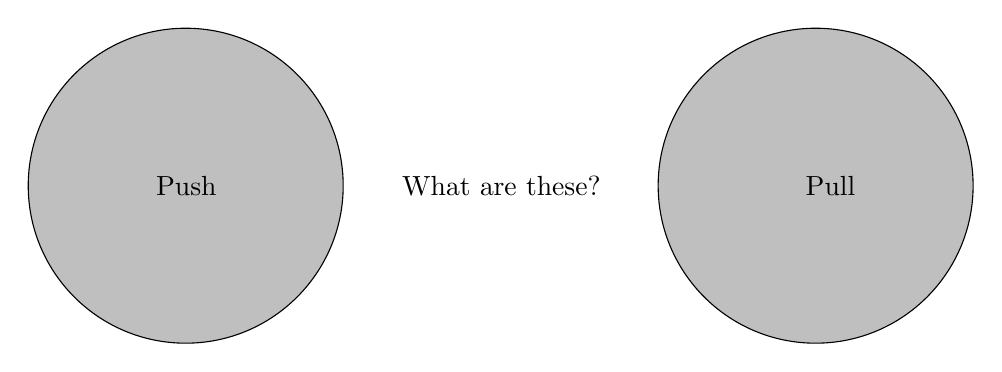
\begin{tikzpicture}
\filldraw[fill = lightgray, draw = black] (4,0) circle (2cm);
\filldraw[fill = lightgray, draw = black] (12,0) circle (2cm);
\draw[black] (3.5,0) node[anchor=west] {Push};
\draw[black] (11.75,0) node[anchor=west] {Pull};
\draw[black] (6.625,0) node[anchor=west] {What are these?};
\end{tikzpicture}
\newpage
\subsection{Newton's First and Second Laws}
\begin{tikzpicture}
\draw[circle] (0,0) circle (0.00001cm);
\draw[->] (3,0) -- (9,4);
\draw[dashed] (3,0) -- (9,0);
\draw[dashed] (9,0) -- (9,4);
\draw[black] (6,-0.5) node[anchor=west] {$F_x$};
\draw[black] (9,1.75) node[anchor=west] {$F_y$};
\draw[black] (5.5,2.5) node[anchor=west] {\begin{turn}{30} $\vec{F}$ \end{turn}};
\end{tikzpicture}
\newline
When we want to start talking about Newtonian dynamics, we first want to define what exactly this term means. We can think of dynamics as being what happens when we have a set of objects imparting certain forces on each other. This is different from kinematics where we are given information about the motion of the objects, and our goal is to describe this motion more thoroughly. I am sure you have heard of Newton’s three laws, and they are very relevant in this discussion. We will now discuss the first one. The first law says that a body undergoing constant velocity motion(which could include being at rest), will stay in this state unless acted upon by force. This means that an object could be going extremely fast, and if nothing goes to slow it down, it will continue at that pace. When I first heard of this law, I found it extremely counter-intuitive. The first reason was that when I was younger, I had always heard that bodies would try to slow down. This was incorrect. As weird as it may seem, it is well tested and documented that objects will not change their speed unless acted upon by an external force. Let us think about some of the consequences this. The first idea is that if we were to have anybody moving at a constant speed $v$ the net force acting on the object must be 0. We can also think about the ramifications if a force is zero in one direction but non-zero in other directions. For now, all we know is that in the direction in which the force is zero, the velocity in that direction must stay constant. We can apply this to free fall. A body undergoing free fall has a force acting on it in the y-direction, but not in the x-direction, so its x-velocity stays the same. 

After discussing the rather qualitative first law, we can now garner a quantitative understanding of the connection between forces and changes in velocity with Newton’s second law. Newton’s second law is deceptively simple. Often we will get problems where we are told to use Newton’s laws. However, often, the insight that allows us to solve the problem will not come from Newton. Newton’s Second law states that the force imparted on an object is equal to its change in momentum over a change in time. For now, we can think of momentum as being the mass(which we will assume to be constant) of a body times the velocity of the body, which we can assume will be changing. So what is the change in mass times velocity divided by a change in time? Well, this is just the mass times the acceleration. From here we get the famous equation. \begin{equation}\vec{F}=m\vec{a}\end{equation} First, we note that acceleration is a vector, so the force is a vector as well. The relation holds in the $x,y$ and $z$ directions and, fundamentally in every direction. We will use this fact later. Another thing to note is how we can derive the first law from the second law. If we set the acceleration equal to 0, we will see that $F=0$. This relation works the other way. If the force is 0, the acceleration must be as well. This is important to conceptualize because questions involving this idea are brought up very frequently. Another important thing to remember is that \begin{equation}\vec{F_{net}}=m\vec{a}\end{equation} $F_{net}$ represents the vector sum of all of the forces acting on an object. So, if there is a force of $F_1$ acting in the I direction on an object and a force of $F_1$ acting in the -I direction, the body will experience no force in the I direction. These are fundamental concepts, and if you do not understand them, I would recommend for you to reread this section. Lastly: Please note that the units of a force are the units of the mass times the units of acceleration. Normally we take this as being $kg \ \frac{m}{s^2}$. However, because physicists like to be concise, this is almost always written using a $N$, for newtons. 

\subsection{Newton's 3rd Law}
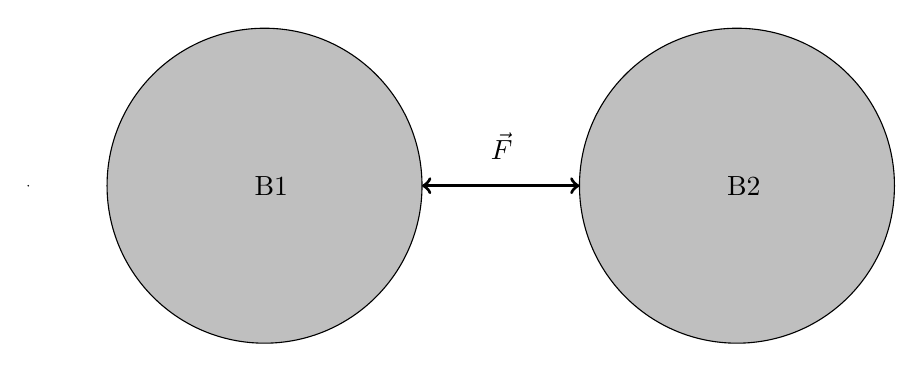
\begin{tikzpicture}
\draw[black] (0,0) circle (0.001cm);
\filldraw[draw = black, fill = lightgray] (3,0) circle (2cm);
\filldraw[draw = black, fill = lightgray] (9,0) circle (2cm);
\draw[very thick, <->] (5,0) -- (7,0);
\draw[black] (5.75,0.5) node[anchor=west] {$\vec{F}$};
\draw[black] (2.75,0) node[anchor=west] {B1};
\draw[black] (8.75,0) node[anchor=west] {B2};
\end{tikzpicture}
\begin{center}
(Figure 3.3.1)
\end{center}

When I was first learning physics, I found the first and second law to be much easier to conceptualize than the 3rd law simply because the first two laws seemed more mathematical. The phasing of the third law in popular parlance is "every action has an equal yet opposite reaction." I frankly believe this is a terrible way to describe the third law. Firstly, it is not at all clear what action and reaction are. Also, we are doing physics here, not chemistry, why are we talking about reactions? The best description I have is that when a body B1 imparts a force  $\vec{F_1}$ on another body(B2). Body B2 must impart a force of magnitude $\vec{F_1}$ but in the opposite direction of $\vec{F_1}$. Please note that this does not refer to a net force, this is only about special forces between objects. One thing the third law tells us is that forces work in both directions. A body can not impart a force on another object without the other body imparting a force on it. This has no parallel in our lives. When we push against something, we do not think of it imparting a force on us but as counter-intuitive as it may seem, this is in fact what is happening. Another interesting example is gravity. The earth acts on us with the force of gravity, and we impart the same force on us. However, because the earth is so massive, our force does not do anything substantive to the earth. $\vec{F} =m\vec{a}$. The force earth imparts on us has magnitude $F$ and causes are the acceleration of $\frac{F}{m}=a=g$. However, The magnitude of the force $F$ is the same for earth but $m_{Earth}$ is much greater than $m_{normal object}$ so $$a_{Earth}=\frac{F}{m_{Earth}}\approx0$$ for all practical considerations.
\subsection{Frictional Forces}
Friction is a difficult concept in elementary physics because it is the first type of non-conservative force that is often taught. The definition of a non-conservative force can be given by using multivariate calculus, or through a relatively simple physical explanation. If you have seen multivariate calculus, then a non-conservative force is a force that has a curl of 0. However, I assume most have not seen this, so, in a physical sense, a non-conservative force is a force that will do non-zero work if you move an object on a closed path(a loop). We will explore this topic furthermore when we talk about work, but for now, we think of friction as something that acts against the motion of an object regardless of whether the object is moving forward or backward. The reason why friction is not conservative we will not discuss technically. However, I think it is important you understand that friction, like the normal force, is the result of intermolecular forces at the layer between the two surfaces. Another important thing to understand is that the frictional force on an object is not constant. The frictional force on an object will increase until it reaches a certain peak amount which it stays at, or it may decrease from if enough force is applied to overcome the frictional force and cause the object to begin moving. For right now, we will discuss the frictional force when the object is not moving. This is called the static frictional force. To help us imagine the static force, I want you to imagine a block on a surface that is being pulled by force in one direction(F) and friction is working against the force. What must the value of the frictional force be? Well, if the acceleration of the body is 0(as it is at rest). Then  \begin{equation}F_{net}\left(x\right)=ma=0=F-F_{friction}\end{equation} The frictional force must take on the value of the force being applied to the object. And then, say that we all of a sudden drop the force by a certain amount. What happens? Well, physically, nothing should happen, the body should stay at rest. Friction can not cause the body to move in the direction of the frictional force. That would not make any sense. No, the body stays at rest and $F_{friction}$ lowers to the new force being applied to the body. So, when a body is at rest, the force of Friction is equal in magnitude to the force being applied to the body, but opposite in the other direction. So what happens as the force being applied to the body increases? Well, the frictional force can’t keep increasing forever, and it doesn’t. It increases up to a certain point after which any added force will cause the body to move. 

Kinetic friction is the friction that occurs when a body is moving.  Kinetic friction is perhaps easier to understand than static friction because, for our purposes, we can assume kinetic friction is not changing if we have a force being applied that is parallel to the frictional force. We saw kinetic friction when we did the example with the block moving down the ramp. The effect of friction was in the opposite direction of the force causing the motion and was perpendicular to the normal force.

Now that we understand the types of friction we can begin to discuss the value of the frictional force for dynamics problems. First, a fact is that the frictional force will vary linearly with the normal force. I like to think about this as making sense. Imagine we have a plane and a block moving across the plane. If we give the block a mass m, there will be a certain frictional force as the body moves. However, if we were to increase the mass of the block, it would at a molecular level at least “sink in” to the table a bit more due to the gravitational force, forcing the normal force to increase to prevent this. When the block sinks into the table a bit more, there is a larger frictional force as for the block to move at a molecular level; it has to descend into the table. This is certainly not an exact description of what is going on here, but it is a way to rationalize why friction would increase when we have a larger mass(and therefore a larger normal force). In practice, you can ignore this description and think of friction as being caused by inter-molecular bumps that require more energy to overcome the more the surfaces in contact are pushing on each other. 

Now we can attempt to do an example with the frictional force. Imagine that we have a plane on which an object is moving as seen below. 
\newline
\newline
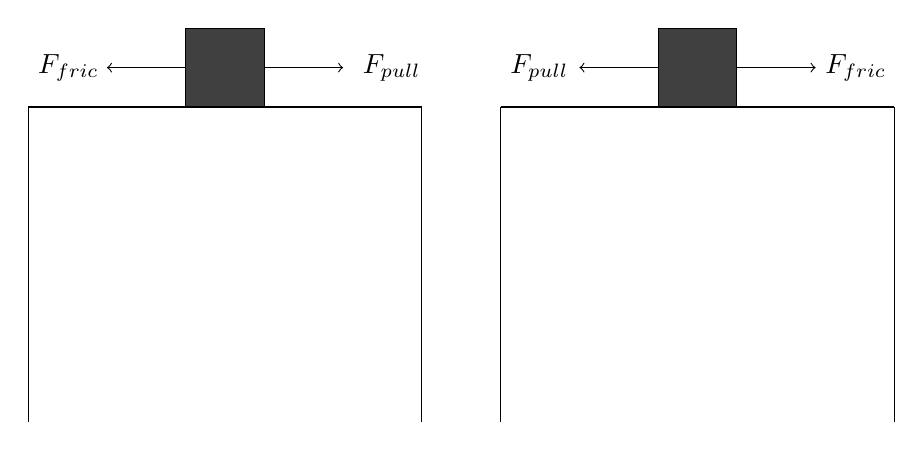
\begin{tikzpicture}
\filldraw[fill = darkgray, draw = black] (2,4) rectangle (3,5);
\filldraw[fill = darkgray, draw = black] (8,4) rectangle (9,5);
\filldraw[fill = darkgray, draw = black] (8,4) rectangle (9,5);
\draw[->] (3,4.5) -- (4,4.5);
\draw[->] (9,4.5) -- (10,4.5);
\draw[->] (2,4.5) -- (1,4.5);
\draw[->] (8,4.5) -- (7,4.5);
\draw[black] (4.125,4.5) node[anchor=west] {$F_{pull}$};
\draw[black] (0,4.5) node[anchor=west] {$F_{fric}$};
\draw[black] (6,4.5) node[anchor=west] {$F_{pull}$};
\draw[black] (10,4.5) node[anchor=west] {$F_{fric}$};
\draw[black] (0,0) -- (0,4);
\draw[black] (0,4) -- (5,4);
\draw[black] (5,4) -- (5,0);
\draw[black] (6,0) -- (6,4);
\draw[black] (6,4) -- (11,4);
\draw[black] (11,4) -- (11,0);
\end{tikzpicture}
\newline
A person is pulling it across the plane and a crane pulling the object up. We can assume that the object is only moving along the plane and not upwards. So we have a classic dynamics problem. We can use Newton’s laws in the x and y directions to create equations of motion that we can use here to find out how fast the object moves given the mass of the object. We are given $\vec{F_{Person}}$, $\mu_{kinetic}$, and $\vec{F_{Crane}}$. Here $\mu_{kinetic}$ is the coefficient of friction for a moving object, that is $\mu_{kinetic}\cdot F_{normal} = F_{friction}$ Once you have the equations given by Newton's law you have to use a certain physical insight to be able to solve the problem. So we have that \begin{equation}F_x=F_{person}-F_{friction}=ma_x\end{equation} and that \begin{equation}F_y=F_{crane}+F_{normal}-F_{Gravity}=ma_y\end{equation} However we know that $a_y=0$, $F_{gravity}=mg$, and that \begin{equation}F_{friction} =\mu F_{normal}\end{equation} So we can write that \begin{equation}0=F_{crane}+F_{normal}-mg\end{equation} And that \begin{equation}ma=F_{person}-\mu F_{normal}\end{equation} From these equations, we see that we know everything we need to find the acceleration other than the normal force. We can use the Eq. 3.4.2. to find the normal force through some simple algebra. We rearrange to find that $F_{normal}= mg-F_{crane}$. Plugging this into the Eq. 3.4.6, we get that \begin{equation}ma=F_{person}-\mu\left(mg-F_{crane}\right)\end{equation} and then we get that \begin{equation}a = \frac{F_{person}+F_{crane}}{m}-\mu g\end{equation} This is very interesting, and we should see if it makes physical sense. First, we see that if $\mu$ were to increase, then the acceleration would decrease. This makes sense because if $\mu$ were to increase, there would be a larger frictional force slowing down the object. We also see that if the mass of the object were to increase we would have a lower acceleration. This makes sense following the law of inertia. We also see that if $F_{person}$ were to increase, then the acceleration of the body would increase. This should also make sense. If there is a larger force pulling on the object trying to move it, then naturally we would have a larger acceleration. Lastly, if the force of the crane were to increase, then we would have a larger acceleration as well. We can rationalize this by looking at the equations which give us some physical insight into why this is. With the equations, we see that if the Force of the crane increases then the normal force decreases and therefore the frictional force decreases, causing a small frictional force. This is quite interesting, even though the crane is not even acting in the same direction as the motion of the object, it can still change its acceleration. 

\subsection{Block on a Ramp}

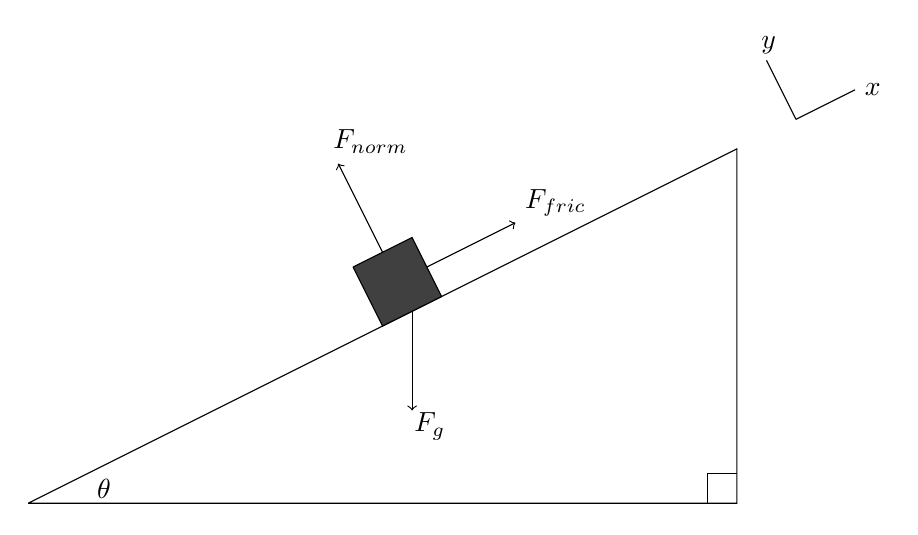
\begin{tikzpicture}
\draw[black] (0*0.75,0) -- (12*0.75,6*0.75) -- (12*0.75,0*0.75) -- (0*0.75,0*0.75);
\filldraw[draw = black, fill = darkgray] (5.5*0.75,4*0.75)--(6*0.75,3*0.75) -- (7*0.75,3.5*0.75) -- (6.5*0.75,4.5*0.75) -- (5.5*0.75, 4*0.75);
\draw[black] (1*0.75,0.25*0.75) node[anchor=west] {$\theta$};
\draw[black] (12*0.75,0.5*0.75) -- (11.5*0.75,0.5*0.75) -- (11.5*0.75,0*0.75);
\draw[->] (6.5*0.75,3.25*0.75) -- (6.5*0.75,1.57*0.75);
\draw[black] (6.375*0.75,1.3*0.75) node[anchor=west] {$F_g$};
\draw[->] (6.75*0.75,4*0.75) -- (8.25*0.75,4.75*0.75);
\draw[black] (8.25*0.75,4.75*0.75+0.25) node[anchor=west] {$F_{fric}$};
\draw[->] (6*0.75,4.25*0.75) -- (5.25*0.75,5.75*0.75);
\draw[black] (5*0.75,6.125*0.75) node[anchor=west] {$F_{norm}$};
\draw[black] (13*0.75,6.5*0.75) -- (14*0.75,7*0.75);
\draw[black](14*0.75,7*0.75) node[anchor=west] {$x$};
\draw[black] (13*0.75,6.5*0.75) -- (12.5*0.75,7.5*0.75);
\draw[black] (12.25*0.75,7.75*0.75) node[anchor=west] {$y$};

\end{tikzpicture}
\begin{center} 
(Fig. 3.5.1)
\end{center}
There are a countless number of dynamics problems that are out there and many of them you will be tested on. The classic ones are problems relating to objects going down ramps, being attached to springs, and being pulled by pulleys. We will go through some of these examples here and present a few other ideas. Fig. 3.5.1. depicts a drawing of a block that has been placed onto a ramp at an angle theta. There are a few things to note here. The first is that the force of gravity points directly down. This makes sense because we can assume the ramp is being placed flatly on earth. Next, we note the force of friction. It is pointing up, and this should be intuitive as we can assume that the block is currently moving down the ramp. Friction, as you know in your daily life, opposes the direction of motion. For now, that is all you need to know. Because the block is going down the ramp, the force points in the exact opposite direction of the motion. The last thing to note here is the direction of the Normal force. In the examples we have seen before, the Normal force is directly opposing the force of gravity, but this is not the case here. Here the normal force is directed perpendicular to the surface of the ramp. This is the nature of the Normal force. The Normal force will always point directly perpendicular to the surface area at which the block and the surface under the block(in this case the ramp) intersect. So if the ramp were completely horizontal, the force would point directly upward and if the ramp was completely vertical. The normal force would be completely horizontal. I like to conceptualize the normal force by imagining, in this case, that the ramp is to be made out of memory foam. If this was the case, the block would slightly come into the memory foam and deforms it. I like to think about the normal force as being the thing preventing this from happening at all(there still is a normal force in the case of memory foam, but it is different than in the case of the wooden block. Now that we are armed with these facts we will use some facts from trigonometry and Newton's laws to determine the motion of the block. We have to use trigonometry here because the forces are not directly perpendicular to each other, such that we can consider them to be acting in entirely different directions, or directly parallel, in which case we can use vector addition. The first thing we have to do is notice that the force of friction and the normal force are perpendicular to each other. This is helpful because we can keep us from having some trouble if we define the direction in which the friction acts(and also the direction of acceleration of the block as being the x-axis and the direction of the normal force as being the y-axis. Now we have to find the components of the force of gravity in the x and y directions. 
\newline
\newline
\newline
\begin{tikzpicture}
\draw[black] (0,0) -- (12,6) -- (12,0) -- (0,0);
\draw[black] (1,0) arc (0:28:1);
\draw[black] (1,0.25) node[anchor=west] {$\theta$};
\draw[black] (6.5,3.25) -- (6.5,0);
\draw[black] (12,0.5) -- (11.5,0.5) -- (11.5,0);
\draw[black] (6.5,0) -- (5.2,2.6);
\draw[black] (5.2,2.6) -- (5.4,2.7) -- (5.5,2.5) -- (5.3,2.4)    --(5.2,2.6);
\end{tikzpicture}
\begin{center} 
(Fig. 3.5.2)
\end{center}
As we can see in Fig. 3.5.2. We can draw a set of three triangles that will allow us to determine the $x$ and  $y$ components of the gravitational force. I will leave it as an exercise to the reader to find these components because it comes up very frequently and is a simple enough application of trigonometry that you should be able to find it on your own. However, as a disclaimer, it is a bit difficult. I will take the result that
\begin{equation}F_{g,x}=F_{g}\sin\left(\theta \right)\end{equation} and likewise \begin{equation}F_{g,y}=F_{g}\cos\left(\theta\right)\end{equation} Armed with these facts, we can now find the motion of the block. The first thing we have to realize is that we can separate $\vec{F}=m\vec{a}$ into the x and y directions such that $F_x=ma_x$. And  $F_y=ma_y$.  So we have \begin{equation}F_x= F_{g}\sin\left(\theta\right)-F_{friction}\end{equation} using the fact that the force of gravity in the x-direction is in the positive x-direction and the force of friction is in the -x-direction. We also have that \begin{equation}F_y=F_{normal}-F_{g}cos\left(\theta\right)\end{equation} Now that we have used Newton's laws, we have to use our physical insight to solve the rest of the problem. Just using the facts we have so far would not be enough to solve the problem. We have to recognize that the force in the y-direction must be 0 because the acceleration in the y-direction is 0. Think about this for a few seconds. Look at how we have defined the y-axis; this should make sense. The object is moving directly along the x-axis here; there is no y-motion. This is only counter-intuitive at first because we are used to thinking that if there is a downward motion, then there must be a y-acceleration. Of course, we have defined the y-axis differently here so this is not the case. Now we have that \begin{equation}0=F_{normal}-F_{g}cos\left(\theta\right)\end{equation} But the force of gravity is just $mg$ so we have that $$F_{normal}=mgcos\left(\theta\right)$$ Now we have to use Newton’s laws in the x-direction. We have that  $$F_x=F_{g}\sin\left(\theta \right)-F_{friction}$$ We know that the Force of gravity is just $mg$ and that $F_x=ma$. I am just writing $a$ here because of $a_y=0$. So $$ma=mg\sin\left(\theta \right)-F_{friction}$$ We can take $\mu$, the coefficient of friction, as a constant that is given to us. So we have that $$ma=mg\sin\left(\theta \right)-\mu F_{normal}$$ And that $$F_{normal}=mgcos\left(\theta \right)$$ If we multiply both sides of this second equation by $\mu$ we have that $$\mu F_{normal}=\mu mg\cos\left(\theta \right)$$ We can plug this new result into our first equation. We have that \begin{equation}ma=mg\sin\left(\theta \right)-\mu mgcos\left(\theta \right)\end{equation} We can cancel the mass out and factor out the $g$ to find that \begin{equation}a=g\left(\sin\left(\theta \right)-\mu cos\left(\theta \right)\right)\end{equation}Often times once we find out a result like this we need to test at edge cases where we can use our intuition to verify the result. This is necessary to verify that our equation is correct, although it does not prove that it is correct. If we say that $\theta=90^o $. We have that $a=g\left(1-\mu \theta \right)$. This means that $a=g$. This should be intuitive to us. If $\theta=90^o$ we have a completely vertical ramp, so the block is just undergoing free fall while next to the ramp. I encourage you to go through this example again because problems relating to ramps occur very frequently on the AP exam. 

\subsection{Pulleys and Tension}

A large number of elementary physics problems include problems with pulleys and with ideas surrounding tension forces. Frankly, I think that these are some of the easier problems on the AP Physics exam and in elementary physics in general. Let us examine the classic problem of two blocks of mass m and M on opposite ends of a massless string being overlaid on a massless pulley in Fig. 3.6.1. These are strong assumptions, but they are made frequently. For now, we have to assume these facts. We can assume that the pulley is being held up by something and is not going to move. Now we want to think about what is going to happen here. Physically, your intuition should be pretty clear. The larger mass should fall down and while doing so pull up the smaller mass. If this was your intuition, very good! If not, I would recommend thinking about this for a few minutes before we get to the equations. 
\newline
\newline
\begin{tikzpicture}
\draw[black] (0,0) circle (0.001cm);
\draw[black] (6,0) circle (1cm);
\draw[black, ->] (8,0.25) -- (8,-3);
\draw[black, ->] (4,-3) -- (4,0.25);
\draw[black] (5,0) -- (5,-3);
\draw[black, ->] (7,-2);
\draw[black, ->] (5,-2);
\draw[black] (7,0) -- (7,-3);
\draw[black] (6.75,-3.75) node[anchor=west] {$M$};
\draw[black] (4.75,-3.5) node[anchor=west] {$m$};
\draw[black] (5.5,-3) rectangle (4.5,-4);
\draw[black] (7.75,-3) rectangle (6.25,-4.5);
\end{tikzpicture}
\begin{center} 
(Fig. 3.6.1)
\end{center}
Armed with this intuition, We can write the equations of motion for the two masses. We can assume that the force of tension acting on both of the masses will be the same. We will take that the positive direction is in the direction of the pulley and the downward direction will be in the direction of the gravitational force. We can then write that \begin{equation}ma_1 = F_{T}-mg\end{equation} and \begin{equation}Ma_2 = F_T-Mg\end{equation} If you do not see why this is, look at the diagram and draw free-body diagrams. We have these two equations, and we are trying to solve for the accelerations of the two blocks. At this point, you may be thinking that we need to be given the tension force to solve for $a_1$ and $a_2$, but this is not the case. To solve this problem, we need to have a physical insight into the nature of a pulley. How can we relate the accelerations of the two pulleys? Think about what is happening as the blocks are going up and down. What must be the case? If you have thought about this for a few minutes, or if you found it immediately, I encourage you to solve the rest of the problem on your own, if not, I recommend you think about it until you find it. 

The insight is that $a_1=-a_2$. Why must this be the case? Because for every inch the less massive block goes up, the more massive block must go down by an inch. This is simply because the string has a fixed length. So we can write \begin{equation}L_1+L_2=L\end{equation}where $L$ is the length of the string, and $L_1$ and $L_2$ are the distances from the masses to the top and middle of the pulley, market point $A$. $L$ is a constant so we can differentiate both sides with respect to t to find that \begin{equation}\frac{dL_1}{dt}+\frac{dL_2}{dt}=0\end{equation} We can differentiate again and rearrange to find that \begin{equation}\frac{d^2L_1}{dt^2}=\frac{-d^2L_2}{dt^2}\end{equation} But wait, $\frac{d^2L_1}{dt^2}$ is just the acceleration of $m$ and $\frac{d^2L_2}{dt^2}$ is just the mass of $M$. This may seem like a rather silly way to come to this conclusion, but if you did not have the original physical insight, you could have found this fact about the accelerations as we have shown. Now we can go about solving the problem. We write that $$ma_1=F_{Tension}-mg$$ and \begin{equation}-Ma_1=F_{Tension}-Mg\end{equation} So if we subtract that second expression from the first one we find that \begin{equation}a_1\left(m+M\right)=\left(M-m\right)g\end{equation} So we finally find that $$a_1=\frac{\left(M-m\right)g}{\left(m+m\right)}$$ And therefore $$a_2=\frac{g \left (m-M\right)}{\left(m+m\right)}$$ This is a classical result in elementary physics, and I find it quite satisfying. However, we should still check it to see if it matches with our intuition. First, let us look at what happens if $M>m$. Then $a_1$ is positive and mass $m$ moves up while $a_2$ is negative and mass $M$ moves down. This is intuitive. If we have two masses and one is smaller, then the larger one should go down while the smaller one goes up. This train of logic works the same if $M<m$. I encourage you as a personal exercise now to find the tension force that the string imparts on the two objects. Also, I want you to find another way you could have solved the problem. A hint would be that it plays with our fixed notions as up and down as necessarily being distinct. This way of solving the problem allows the direction of a curve to be positive and the opposite direction of the curve to be negative. This way of solving the problem is quite a lot easier, and I think you will gain quite a bit from thinking about it on your own. 
\clearpage

\subsection{Centripetal Force and Acceleration}
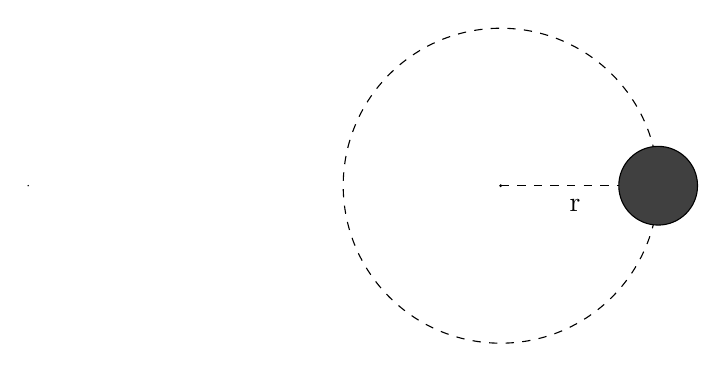
\begin{tikzpicture}
\draw[black] (0,0) circle (0.0001cm);
\draw[dashed, draw=black] (6,0) circle (2cm);
\draw[dashed, draw=black] (6,0) circle (0.01cm);
\draw[dashed, black] (6,0) -- (8,0);
\draw[black] (6.75,-0.25) node[anchor=west] {r};
\filldraw[fill = darkgray, draw=black] (8,0) circle (0.5cm);
\end{tikzpicture}
\newline

Now that we have dealt with linear motion, we need to deal with centripetal(circular) motion. There are only a few things you need to know about centripetal forces, but once you know the first few things, we will be able to do quite a lot. The first thing you need to know is when we can talk about centripetal force, motion, and acceleration. We should discuss centripetal motion when an object is moving in a circle. We do not want to think about centripetal force in the same way here as when an object is rotating about an axis inside of it. For example, if we think about the earth circularly going around the sun, we can discuss centripetal force. Meanwhile, if we think about a fidget spinner rotating around its center, we can not think about centripetal force. However, if we were to think about one small slice of one blade of the fidget spinner moving about in a circle, we could think about centripetal force. Hopefully, these examples will give you the idea. Later, we will discuss rotational motion, and as you will see, there are connections between rotational and centripetal motion, as essentially, they describe the same concepts.

Next, we need to think about what centripetal motion we will study entails. For us, centripetal motion is when an object is rotating around in a circle with a constant speed. So, what is different about centripetal motion compared to accelerating linear motion is that centripetal motion involves the magnitude of velocity(speed), staying constant, while the direction of the velocity is changing. This means that $\frac{dv}{dt}$ is not zero, because $\vec{v}$ is a vector and its direction is changing. Next, we need to think about the magnitude of the acceleration that is being produced in addition to the direction of the acceleration that is being produced. I am going to spare the details of the proof here because I believe they involve more mathematics than physics. However, I would still recommend you search for the proof yourself because it is beneficial to know exactly why this formula is true because it is ubiquitous. The formula is that \begin{equation}a_c=\frac{v^2}{r}\end{equation} with $a_c$ representing the magnitude of the centripetal acceleration and $r$ being the radius of the circle that is formed by the movement of the object. You also need to know that the centripetal acceleration is directed directly towards the center of the circle that the object is moving around. I am going to give a sort of proof by contradiction as to why this is true. First, remember that the velocity of an object moving around in a circle is directly tangent to the point along the circle that the object is in. This is because the velocity of an object must always be tangent to the path of its motion, by definition. Next, imagine that the acceleration had a component in the direction tangent to the circle. Then, the velocity of the object would increase or decrease. But we have said that the velocity of the object is remaining the same when undergoing centripetal acceleration. This is a contradiction. So all of the centripetal acceleration must be pointed towards the center of the object's path. This direction is called the radial direction. Now that we have an understanding of the direction of the centripetal acceleration, we should try to justify why the formula would be true physically. First, let us think about why $a_c$ should be larger when we have a larger velocity. This is because if the velocity is higher, a larger acceleration is required to switch the direction of the velocity faster(assuming a constant radius). Next, we need to think about why increasing the radius would decrease the centripetal acceleration. This is because when we have a larger radius, the object “has more time” to modify its velocity. If you are not satisfied by these explanations(as I was at first), I recommend you go through the mathematical derivation which should only serve to strengthen your physical intuition. 
Now that we know the formula for centripetal acceleration, we need to understand how it applies. You may be having a question now, what even is centripetal acceleration? Well, essentially, centripetal acceleration is the acceleration in the inward radial direction that is required for an object to go into a circle. So essentially, it is a real requirement, but forces do not cause a centripetal acceleration only. This sounds kind of silly so let us go through a real example to strengthen this idea. 

The classic example is a block on a string that is swirling in a circle in a vertical plane. Imagine that the string is the black line and that the rightmost endpoint of the string is being held constant in space such that the entire string is rotating in a circle. Let me give you a challenge now. If we say that the object has a mass m, is in rotation at a constant velocity of v in the plane with a circular trajectory of radius r, what is the value of the tension in the string holding the object as a function of the angle $\theta$(you only need to do this when the mass is above the rightmost end of the string and to the left of the center of the string)? The AP Exam will probably only ask you about this at the highest and lowest points of the circular trajectory of the mass, so I recommend that you find these as well. 

Now that you have either solved the problem or if you can’t seem to figure it out, let us use Newton’s laws to solve this problem. Remember that the direction of the centripetal acceleration is always vertically inward(which the tension also is, and which a component of the force of gravity is. We discussed how to find the component of the force of gravity earlier, so I will not discuss it here and recommend that you go back to the slanted plane lesson earlier to see this discussion. We have that the component of the force of gravity in the inward radial direction is $$mg\sin\left(\theta \right)$$ So we need to add the gravity and tension together to find the total force on the object in the inward radial direction, we find that \begin{equation}T+mg\sin\left(\theta \right)=F_c\end{equation} But $F_c=ma_c$, and $a_c=\frac{v^2}{r}$. because the direction of the centripetal acceleration behaves like any other direction in the eyes of nature. So we have that \begin{equation}T=\frac{mv^2}{r}-mg\sin\left(\theta \right)\end{equation} That is our entire expression because everything is constant other than $\theta$. Hopefully, this example showed how to deal with forces so we can use our formula for centripetal acceleration to our advantage. 
\subsection{Mass and Physical Definition of Weight}

One of the most classic things people learn when they take introductory physics is the difference between mass and weight. Unfortunately, the way that the concept is taught is often in a rather silly way that hinges on diction rather than having any real physical insights. The idea of what mass is is fairly simple. In physics, mass is described by the amount of matter a certain thing has. It is important to understand that of the fundamental forces of physics(you do not have to know these), gravity is the only one that relies on mass to determine its strength. So in a physical sense, mass is measured by measuring the force that acts on a body in a known gravitational field. This is a circular definition, but it can help us better understand mass when compared to trying to figure out what exactly “matter” is. Now that we have a better grasp of what exactly mass is, we can give a proper definition of weight. In our popular use, we use weight as the same as mass, and that is correct in popular parlance. However, physicists define weight differently. Physicists define weight as the product of the acceleration of free fall times the mass of the object. This is equal to the gravitational force acting on an object and is denoted as either $$W$$ or $$F_G$$ This may seem odd because it gives us a definition of weight that is in Newtons rather than pounds or kilograms. This definition of weight is one common definition, but, on certain problems and  physics books, the weight of an object is the weight that you will get if you put an object on a scale while it undergoes some force. The value that you record on the scale(which will be the force that the scale imparts on the person), will be the weight of a person. We are asked for this type of weight very frequently. Sometimes this weight is called apparent weight, and it is ubiquitous in cases in which a body is submerged in liquid or is experiencing net acceleration not being entirely caused by gravity(as in the case of a moving elevator). Now let us consider this example of a person standing on a scale in an elevator. Our job is to find the weight recorded on the scale. Now, we will formally introduce the free-body diagram. 
\begin{tikzpicture}
\draw[black] (0,0) circle  (0.0001cm);
\draw[black] (4,0) -- (4,6) ;
\draw[black] (4,0) -- (8,0) ;
\draw[black] (8,0) -- (8,6) ;
\draw[black] (4.5,0) -- (4.5,0.5);
\draw[black] (7.5,0) -- (7.5,0.5);
\draw[black] (4.5,0.5) -- (7.5,0.5);
\draw[black] (4.75,0.5) -- (4.75,2);
\draw[black] (7.25,0.5) -- (7.25,2);
\draw[black] (7.25,2) -- (4.75,2);
\draw[black, ->] (6,2) -- (6, 4);
\draw[black] (5.75,4.25) node[anchor=west] {$F_N$};
\draw[black, ->] (6,0.5) -- (6, -1.5);
\draw[black] (5.75, -1.75) node[anchor=west] {$F_g$};
\draw[black, ->] (3,6) -- (3,0);
\draw[black] (2.75,-0.125) node[anchor=west] {$a$};
\end{tikzpicture}
\
\newline
A free-body diagram is a simple way of diagramming the forces acting on an object. Here we take the box to be the person for simplicity. We have been seing this before but in this section, when a more detailed analysis is required, we will give it a formal name. The force of gravity and the force of the scale on the person are opposing each other and result in the net downwards acceleration. Now that we have identified the forces acting on the person, we can use Newton's laws to determine the force the scale is exerting on the person. We will take the downwards direction as being positive. This means that \begin{equation}ma=mg-F_{Scale}\end{equation} This means that \begin{equation}F_{Scale}=m\left(g-a\right)\end{equation} It is interesting to see from this equation that if the downwards acceleration of the elevator is equal to $g$, then the scale will record the weight of the person as being 0. This is what happens in zero-gravity simulating planes. 


\subsection{Systems Analysis}
Lots of dynamics problems are easily solved once we have a set of physical insights about what is happening in the problem. At least, this is the case for the more interesting problems. However, for many AP Physics problems, the way to solve the problem is to recognize the formula that you need to use. It is remarkable how many problems are of the form "imagine that such and such is increased/decreased by a factor of such and such, what happens to such and such?". These problems simply require looking at or recalling the necessary equations and using them. In this section, however, I instead want to focus on some tricks that can help you with more complex problems. The first is to recognize that there are multiple ways of looking at problems. One way is to adopt a "systems approach". It is useful to adopt a systems approach to problems where we have more than one body interacting. This way of thinking can help shorten your calculations significantly and is necessary for more complex problems. By thinking about a group of bodies as a system, I mean to look at all of the bodies as a whole and not to think  about how they are interacting with each other. This is better seen than read, so let us do an example. 

\
\newline
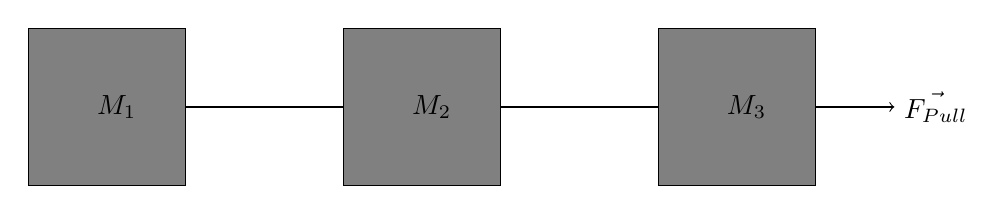
\begin{tikzpicture}

\filldraw[draw= black, fill = gray] (0,0) rectangle (2,2);
\filldraw[draw= black, fill = gray] (4,0) rectangle (6,2);
\filldraw[draw= black, fill = gray] (8,0) rectangle (10,2);
\draw[black] (2,1) -- (4,1);
\draw[black] (6,1) -- (8,1);
\draw[black, ->] (10,1) -- (11,1);
\draw[black] (0.75,1) node[anchor=west] {$M_1$};
\draw[black] (4.75,1) node[anchor=west] {$M_2$};
\draw[black] (8.75,1) node[anchor=west] {$M_3$};
\draw[black] (11,1) node[anchor=west] {$\vec{F_{Pull}}$};
\end{tikzpicture}
\newline
\begin{center}
(Figure 3.9.1)
\end{center}
In Fig. 3.9.1 we see that the three blocks are being pulled by a pulling force. We can imagine that the strings between the blocks are rigid and do not move and are fixed to the blocks. So the blocks are being pulled uniformly. Our task is to find the acceleration of the system. We may assume the rods to be massless. When I first saw a problem like this, I was quite confused. I found it weird that the $M_1$ seemed to have nothing pulling on it but it must have still been moving. However, I was wrong in thinking that there is no force acting on the first $M_1$. The rod between $M_1$ and $M_2$ is pulling on $M_1$ and causing it to move. Additionally, the rod between $M_1$ and $M_2$ is exerting a tension force on $M_2$, but the force is in the opposite direction of $F_{Pull}$. If this confuses you. Think about a small fraction of the rod. It has a net force of 0 acting on it. Why? Because even though it has an acceleration, the mass is 0. So, there is a tension force acting both ways. The same ideas apply for the rod between the 2nd and 3rd masses. We can use Newton’s laws to write equations, and we will be able to find the acceleration, but there is a smarter way. It utilizes the fact that the blocks are moving in parallel, and it is not a particularly complex idea. The simple truth is that we treat the entire mas-rod system as a big system. We can do this because the mass-rod system is connected and will move with one acceleration. We say that $$F_{Pull}=Ma$$ Where $M$ is the mass of the system. Well, what is $M$? Simple, $M$ is just $$M{system} = M_1+M_2+M_3$$ So \begin{equation}a=\frac{F_{Pull}}{M_1+M_2+M_3}\end{equation}. This result makes intuitive sense, if we increase the pulling force, we would expect the acceleration to increase, and it does. Meanwhile, if we increase any of the masses, the acceleration would decrease, which makes sense. Now that we have seen the systems approach I encourage you to solve this problem without using this and compare to see how powerful this method is. Now, if you are still confused, I want you to think about it in the following way. I did not specify how long the rod was. What if it was tiny, only the length of a few atoms. All of the calculations would be the same as we still have the same ideas, but we could think of it as being one extended block of mass $$M_{block}=M_1+M_2+M_3$$ being pulled. From here, we can think about this as being a one body problem because after all, we could arbitrarily split any given mass into smaller masses and we would essentially have a three-body problem. This is a classical example in physics of thinking about the asymptotic behavior of a formula in order to determine its validity.

\section{Work, Energy, and Power}
\subsection{What is Energy?}
\begin{tikzpicture}
\draw[black] (0,0) -- (0,8);
\draw[black] (0,0) -- (12,0);
\draw[black] (0,8) .. controls (2,2) .. (12,8);
\draw[black] (4,-0.5) node[anchor=west] {$Possible \ Energy \ States$};
\draw[black] (-0.75,3.25) node[anchor=west] {\begin{turn}{90} $Potential \ Energy$ \end{turn}};
\end{tikzpicture}
\newline

We will now begin discussing energy, power, and work after having talked about Newton’s laws and dynamics. These will serve as an alternative to Newton’s laws that we can use to analyze certain situations. When I first began learning about energy, I was plagued by one question: “What the hell is energy.” The description I was given was “the ability to do work.” This definition is correct, but because AP Physics does not deal much with thermodynamics, it is not particularly useful.  I mean, we hardly use energy to think about objects doing work in AP Physics. Instead, we think about energy in terms of forces doing work on objects. Primarily because we will often deal with energies that are negative and in that case, what does having a negative ability to do work even mean. In fact, in chemistry, almost all of the energies that one deals with are negative. So, how should you think about energy in this course? Well, I would recommend thinking about energies in the same way we think about energy in chemistry. Energy is a way of representing how much a system does not want to be the way it is, and subsequently how much work it took for the system to get to the way it is. This is not a technical definition, and we will see the technical definition later but I want you to think about this now, and what types of things would signify a high energy. A few examples would be, a pencil balancing on its pointed end, two positive point charges sitting very close to each other, and a ping-pong ball floating high in our sky. When you think about these examples, one thing should become clear to you; the objects will not stay in these positions. The objects will naturally try to lower their energy. This is why I like thinking about energy as a bad thing, and this description will almost always work for our purposes.  

\subsection{Work and Power}
We will now begin to deal with work and power. I am sure you have heard about work and power because they are some of the only terms in physics that we can see used in our daily lives. The first thing that you have probably learned about work is that \begin{equation}W=Fd\end{equation} First, here W is work, F is the force, and d is the distance that the object has traveled. First, we need to introduce a new unit called the Joule to begin talking about work. A joule is simply a Newton times a meter. Which is $\frac{kg\cdot m^2}{s^2}$. Of course, it is unclear exactly what we mean by Force and distance here and this definition is not true in general, so it is not particularly useful. A better, but still imperfect definition of work is \begin{equation}W=\vec{F} \cdot \vec{d}\end{equation} Where $\vec{d}$ is the vector representing the distance that the object has traveled. This tells us that the work a force does on an object is the dot product times the position vector of the object. If you know what dot products are, then you should be able to reason when the work done by a force is 0 and when it is at a maximum assuming the force is constant. If you have not yet seen the dot product or do not remember it, I will provide a refresher here. $$\vec{a} \cdot \vec{b}=|\vec{a}| \ |\vec{b}| \ \cos\left(\theta \right)$$ $\theta$ here is the angle between the two vectors. What this means is that if $\vec{F}$ and $\vec{d}$ are along the same direction then $\theta$ is 0 and $$\cos\left(\theta \right)=1$$ so the work is just $$\mid \vec{F}\mid \ \mid\vec{d}\mid$$ $\cos\left(\theta \right)$ is always less or equal to 1 so when $\vec{F}$ and $\vec{d}$ lie along the same direction, work is at a maximum. When $\vec{F}$ and $\vec{d}$ vary by an angle of $90^o$ then $\cos\left(90 \right)=0$ and the work done by the force is 0. So, if the Force is 90 degrees off from the distance of the object, then no work has been done by the force. When theta varies from $0^o$ to $90^o$ degrees, the force progressively declines. You may be wondering, what happens when the angle goes beyond $90^o$. Well when the angle increases from $90^o$ to $180^o$, the work becomes negative. It may be weird to think of negative work, but I think of negative work as occurring when a force is trying hard to make an object switch directions but is unable to. In contrast, positive work is when a force tries to make an object move a certain way, and it is effective. 

A question I always had was, what happens when the Force is changing, and the path is not linear or circular? Well, to do this we need to use calculus and to do it and two and three dimensions, we need to use techniques from multivariate calculus called line integrals. However, we do not need to worry about this level of mathematics. Instead, let us imagine that the force is changing with distance but changes very little when we change the distance($d\vec{x}$). So if we change the distance by a very small $\Delta x$, we can approximate the work as $$\vec{F} \cdot d\vec{x}$$ However, a movement from point a to point b requires a whole bunch of small little changes that can be approximated as $$\vec{F} \cdot d\vec{x}$$ So we can use an integral to sum all of these tiny amounts of work to find the real work. Our approximation becomes more and more accurate as $d\vec{x}$ goes very close to 0. So we write that \begin{equation}W=\int{\vec{F} \cdot d\vec{x}}\end{equation} With this formula, we can do problems where we have a force changing in magnitude with the direction of the force and the path always being the same.

I will not present an example that is not particularly realistic but useful for calculation purposes; we shall imagine a force where \begin{equation}F\left(x\right)=4x^3+x^2+1 \ N\end{equation}, and the force is acting on an object that is moving from $x=2$ to $x=4$. We can assume that $x$ and $dx$ have been normalized with respect to meters. Now we can now just say that work is force times distance because the force is changing, but the directions of the two vectors are the same. So we need to use an integral equation. \begin{equation}W=\int x^3+x^2+1 \ dx \ J= \frac{x^4}{4}+\frac{x^3}{3}+x \ J\end{equation} Plugging in from $x=2$ to $x=4$ we find that   $$\left(64+\frac{64}{3}+4\right)-\left(4+\frac{1}{3}+2\right) J= \frac{242}{3} J$$ This means that the force did about 71 Joules of work in moving the object from $x=2$ to $x=4$. 

Now that we have seen what work is through calculations, we need to get an intuitive understanding of what exactly is going on. We can think about work as being something that forces do to cause objects to move as they want them to. When a force does positive work, it successfully moves an object the way that it wants too. When a force does negative work, it has “failed” at getting the object to move as it “wanted” it too. It is, of course, important to recognize that forces don’t “want” anything but this is a good way of thinking about this topic. 

Now that we have introduced work, we need to think about power. Power is the amount of work that is delivered to something per unit time. In terms of calculus $P=\frac{dW}{dt}$ or $P = \frac{\Delta W}{\Delta T}$. If we assume that the force is not changing and that the force is applied in the same direction as the motion of the object, we can write $$P=\frac{d\left(Fr\right)}{dt}$$ We assumed the force is constant so we can take the F term out and we find that $$P=F\frac{d\left(r\right)}{dt}$$ But $$\frac{dr}{dt}$$ is just the velocity of the object, so we can say that $$P=Fv$$ In the more general case where $\vec{F}$ and $\vec{v}$ are not necessarily in the same direction, we have that $P=\vec{F}\cdot \vec{v}$. It can be confusing what exactly the power is here. For clarification, the power we are talking when we write \begin{equation}P=\vec{F} \cdot \vec{v}\end{equation} is the power delivered to the object by force. So, if for example, an object is moving horizontally across the ground on earth. Gravity is not providing any power because the force and the velocity are perpendiculars, so the dot product goes to zero. The intuition for power is pretty simple. For example, imagine a person trying to move an object from point A to point B. They perform the task but the object experiences a lot of friction, and it takes a time $T_1$. Now imagine an alternate reality where the person asks his/her friend to help, and the two of them move the object from point A to point B in time $T_2<T_1$. Because $T_2<T_1$ the two people move the object with more power(together) because the work of moving the object across the floor is constant, but the time has decreased. 

\subsection{Kinetic Energy}
\begin{tikzpicture}
\draw[black] (0,0) -- (0,8);
\draw[black] (0,0) -- (10,0);
\draw[gray] (0,8) parabola (8,0);
\draw[gray] (0,0) parabola (8,8);
\draw[black] (4,-0.5) node[anchor=west] {Time};
\draw[black] (-0.75,3.5) node[anchor=west] {\begin{turn}{90} $Potential \ and \ Kinetic \ Energy$ \end{turn} };
\end{tikzpicture}

Kinetic energy is the so-called energy of motion. This means that when an object is moving, it  will have a certain amount of energy associated with this motion. To be more specific, Kinetic Energy is the energy gained by an object when a conservative force does work on an object. So when a certain amount of work is done on an object by this conservative force, we would expect the kinetic energy of the force to increase or decrease in turn. We can see this if we look at the expression for work. Work is $$\int{\vec{F} \cdot d\vec{r}}$$ By the second law, this is just $$\int{m\vec{a} \cdot d\vec{r}}$$ But $a=\vec{dv}{dt}$ so we can replace that here $$\int{m\frac{dv}{dt} \cdot d\vec{r}}$$ Now we are going to do something not mathematically rigorous but that physicists use all the time and will work fine for our purposes. That is, we are going to say that we can move from under the $dt$ from the $d\vec{v}$ to the $d\vec{r}$. It is if we are treating $dt$ as just another number that we can multiply. Once again, this is not rigorous, but if you think about $dt$ as just a number, you should see why this makes intuitive sense. Now we can substitute $$\frac{d\vec{v}}{dt}d\vec{r}$$ for $$\frac{d\vec{r}}{dt}d\vec{v}$$ But $\frac{dr}{dt}$ is is just $\vec{v}$. So we can rewrite our integral as $\int{mv d\vec{v}}$. When we integrate we use the power rule and then substitute at two velocities to find that find that \begin{equation}W=\Delta\left(\frac{mv^2}{2}\right)\end{equation} we have said that kinetic energy is the change associated in the energy of an object when work is performed on it so from Eqn. 3.4.1 it is clear that $\frac{mv^2}{2}$ is just what we are looking for. Kinetic Energy is often denoted as K, and its units are the same as those of work, Joules. \begin{equation}K=\frac{mv^2}{2}\end{equation} The connection between work and energy that we have just derived is called the work-energy theorem. The work-energy theorem states that \begin{equation}W_{conservative}=\Delta K\end{equation} When I first learned this formula I was amazed because it seemed magical that this term we had created was exactly what we needed in this case. This formula will come in handy in many situations, so it is important that you fully understand it and its derivation. Also, note that this formula can only be applied in one dimension. Because work is a dot product, we would have to use the dot product to find the answer when we have multiple dimensions, and I would challenge you to do this using the same method we have described above. The answer may be less satisfying, but it may help you answer some of the questions you have. Now that we have started talking about the kinetic energy we have to study potential energy. We will study it more rigorously later but for now, think about potential energy as being energy that will later be converted into kinetic energy. So, if a ball is very high, it will have higher potential energy because it will fall farther and hit the ground with a faster speed(and therefore kinetic energy), than a ball that was dropped from a lower height. For our purposes, we only need to consider one type of potential energy this way. That is gravitational potential energy. Essentially, when things get higher in the sky, they get more gravitational potential energy. Likewise, when things get lower, they will lose potential energy. Like always, work and potential energy are closely related. When a conservative force does work on an object(for right now this means gravity), the potential energy of the object will decrease with the same magnitude as the work done on the object. Another way of writing this is that \begin{equation}W_{conservative} = -\Delta U\end{equation} Where $U$ represents the potential energy. All this says is that when gravity does work on an object(by lowering its position), the potential energy of the object will decrease by the same amount. Think about this if you have trouble with it because we will use this definition very often. Now let us think about what happens when the gravitational force does work on an object. The first thing to note is that we can consider the gravitational force to be directly down. This means that if an object moves to the right or left, the gravitational force is not responsible for this movement. So let us think about the work done by gravity on an object that moved down a height $h$. The work done will be $mgh$. This is because the direction of the motion(downwards), and the force of gravity(also downwards), are the same, so the angle is 0 and $\cos\left(\theta \right)=1$. Also, the force is $mg$ and is constant, and the height moved downward is $h$. The product is $mgh$. Therefore if the work is done is $mgh$, the potential energy has decreased by $mgh$ in turn. The opposites would be true if the object went up by a height h. The work done would be $-mgh$, and the potential energy would increase by $mgh$. Hopefully, this will not be too confusing but you should not that I have only defined what a change in potential energy entails and not what the exact value of potential energy is. That is because for what we are doing right now, we can define the absolute value of the potential energy however we would like. For example, if we have an object at a height h above the earth at $t_1$ and the same object on the ground at $t_2$. We could define the potential energy of the object at $t_2$ as 0, and the energy of the object at $t_1$ as $mgh$. This is because the work done by gravity in bringing the object from height h to the ground is $mgh$, so the potential energy from height $h$ to the ground decreases by $mgh$ and therefore the ball must have potential energy greater at height h by $mgh$. However, it is not necessary that this value be $mgh$. All that matters is that the difference in potential energies is $mgh$. So, we could say the potential energy at height $h$ is $2mgh$ and at the ground is $mgh$ . Once again, all that matters is the difference. We will see this one more time when discussing electric potential. Now that we understand potential and kinetic energy, we need to understand the relationship between the two; this comes in the form of conservation of energy. Essentially, the first thing we need to know about conservation of energy is that \begin{equation}K_1+U_1=K_2+U_2\end{equation} if only conservative forces are acting on the system with the energy. Simplifying this we can write that $$\Delta U+\Delta K=0$$ when the only forces acting on the object are conservative. You can get this formula yourself by plugging in the values we have given for $\Delta U$ and $\Delta K$ before. It is easy to see now that we have written the formula for the conservation of energy in this way, what the formula should be when we have non-conservative forces acting on the object. All you need to know about conservative and non-conservative forces now is that gravity is the only conservative force of importance. So anything else will be non-conservative. Essentially, non-conservative forces take energy or add energy to a system, while conservative forces cannot do this. So we can write that \begin{equation}\Delta U+\Delta K=W_{non-conservative}\end{equation} where $W_{non-conservative}$ is the work done on the system(or just object) by the non-conservative force. To illustrate this concept, we will do one example that encompasses all of the topics we have learned about. This is just a block sliding down a frictional plane, as seen in Fig. 4.3.1. Our task is to find out what the velocity of the object will be once it gets to the bottom of the plane. We will be given the angle of the frictional plane, the length of the place, the frictional constant, and the mass of the object. 

Also, we can assume that the object essentially only occupies the exact top of its current location, so we do not have to worry about the fact that it is not completely at this top. This assumption from now is often implicitly made but will not be stated. Also, we assume the mass is at rest at the top of the ramp. We use Eqn. 4.3.6. 
\newline
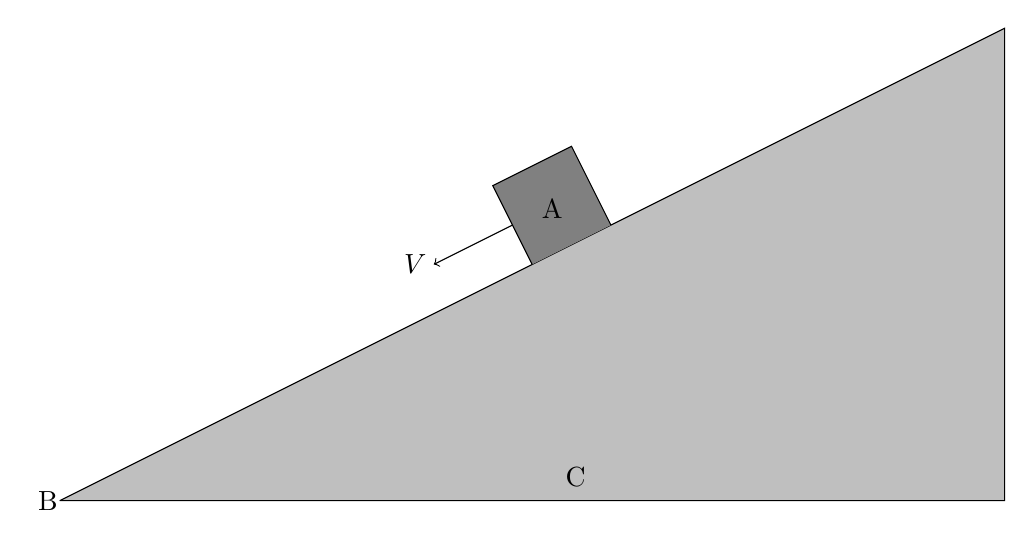
\begin{tikzpicture}
\filldraw[draw = black, fill = lightgray] (0,0) -- (12,0) -- (12,6) -- (0,0);
\filldraw[draw = black, fill = gray] (6,3) -- (5.5,4) -- (6.5,4.5) -- (7,3.5);
\draw[black, ->] (5.75,3.5) -- (4.75,3);
\draw[black] (4.25,3) node[anchor=west] {$V$};
\draw[black] (6,3.7) node[anchor=west] {A};
\draw[black] (6.3,0.3) node[anchor=west] {C};
\draw[black] (-0.4,0) node[anchor=west] {B};
\end{tikzpicture}
\newline
\begin{center}
(Figure 4.3.1)
\end{center}
$$\Delta U+\Delta K=W_{non-conservative}$$ Here, friction will be the non-conservative force. We can calculate what $W_{non-conservative}$ is at the beginning. The normal force is $$mg\cos\left(\theta \right)$$ Therefore the force of friction is $\mu mg\cos\left(\theta \right)$ in the direction up the ramp because the mass is going down the ramp. So the work done by friction is $$\vec{F} \cdot \vec{d}=\mu mgh\cos\left(\theta_1 \right)$$ Here $\theta_1$ is the angle between the force of friction and the direction of motion of the mass. $\theta_1$ is 180 degrees so $cos\left(\theta_1 \right)=-1$ and therefore,  $$W_{non-conservative}=-\mu mgh\cos\left(\theta_1 \right)=\Delta U+\Delta K$$ Next, let us examine the change in kinetic energy. The kinetic energy of the object at the top of the ramp is 0(it is at rest) as. So, $$\Delta K=\frac{mv^2}{2}$$ In this example, and many other examples, the kinetic energy term will allow us to find the velocity of the object. Next, we need to find the change in potential energy of the object between the top and bottom of the ramp. Remember that $$W_{conservative}=-\Delta U$$ So, if we find the work done by gravity in moving the mass from the top to the bottom of the ramp, we will be able to find the change in potential energy of the object. We are going to use something special about conservative forces to find the work done by gravity here. That is, we will use the fact that conservative forces are path-independent. So, the work done by gravity in taking it from point A to point B will be the same as if we took the object from point A, directly down to the bottom of the ramp to point C, and then directly to the right to point B. In moving the object from point C to point B, gravity does no work because it is directly perpendicular to the motion of the object. Meanwhile, gravity does do work while moving the object from point A to point C. And when moving it from A to C, the force of gravity and the direction of motion of the object is in the same direction so $$W_{gravity}=mg\left(distance\ from\ point\ A\ to\ point\ C \right)$$ Using trigonometry(I recommend you do this yourself), we can find that the distance from point A to point $C=h\sin\left(\theta \right)$. Therefore \begin{equation}W_{gravity}=mgh\sin\left(\theta \right)\end{equation} Finally, we have \begin{equation}\Delta U=-mgh\sin\left(\theta \right)\end{equation} So, we can now finally find the velocity we are looking for. $$-\mu mgh\cos\left(\theta \right)=-mgh\sin\left(\theta \right)+\frac{mv^2}{2}$$ We can rearrange this equation to find that $$mg\left(\sin\left(\theta \right )-\mu \cos\left(\theta \right)\right)=\frac{mv^2}{2}$$ Therefore \begin{equation}v=\sqrt{\left(2mgh\left(\sin\left(\theta \right)-\mu \cos\left(\theta \right)\right)\right)}\end{equation} You may be confused as to what happens when $$\sin\left(\theta \right)-\mu \cos\left(\theta \right) < 0$$ If this were the case, the velocity would be an imaginary number. Well, do not worry. This is not possible. If $$\sin\left(\theta \right)-\mu \cos \left(\theta \right) < 0$$ then object will not move initially and our formula will not apply. I challenge you to justify this for yourself using Newton’s laws. 

\subsection{Conservative Forces and Potential Energy}
\begin{tikzpicture}
\draw[black] (0,0) circle (0.0001cm);
\draw[black] (3,1) rectangle (9,6);
\draw[black] (4.125,5) node[anchor=west] {$\oiint_S \vec{E} \cdot d\vec{A} = \frac{Q}{\epsilon_0}$};
\draw[black] (4.125,4) node[anchor=west] {$\oiint_S \vec{B} \cdot d\vec{A} = 0$};'\draw[black] (4.125,3) node[anchor=west] {$ \oint_P \vec{B} \cdot d\vec{r} = \mu_o I + \epsilon_o \mu_o \frac{\partial \Phi_E}{\partial t}$};
\draw[black] (4.125,2) node[anchor=west] {$ \oint_P \vec{E} \cdot d\vec{r} = \frac{-\partial \Phi_B}{\partial t}$};
\end{tikzpicture}
\begin{center}
(Figure 4.4.1)
\end{center}
Above are the Maxwell Equations describing the electromagnetic force. The electric force is conservative while the magnetic force is not. 
As we have already seen in our discussion of potential energy, forces and potential energy are closely related. You will see in electricity and magnetism how electrical potential and electrical potential energy will use some techniques from multivariate calculus to develop these concepts more rigorously. We will think about potential energy only for conservative forces because the concept would not fit with non-conservative forces. For this reason, we will see an electric and gravitational potential energy, but we will not, for example, see a magnetic or frictional potential energy. In case you do not remember, a conservative force is a force for which if a body starts at a given point, and goes on any path and returns the same point, the work done by the force is 0. This must be true for all of the points in the plane. By this I mean, if we move an object from point A to point B regardless of how, the same amount of work must be done by the force. It is path-independent. So, in some sense, we can think about each point having a distinct energy associated with it where the work done by a force in moving it from A to B is the difference between the energy at these points. We will discuss this topic in more detail when we cover gravitation later, and we will discuss how we can think of the gravitational force as being the result of a “force field” that permeates all space. To repeat, if the force is conservative, it does not matter which path for determining the work done. We still have a problem though. How do we assign each point an energy value? If we know $8$ J of work are done in taking an object from point A to point B, how do we determine energy values based off of these? Well, what we can do is to assign a value of 0 for the energy at any location. We usually take this location as infinity, which we think of as being infinitely far away from everything we are considering.

AP Physics only covers the gravitational and electrical forces, as such, we will think about potential energy regarding gravitational and electric forces. It is important not to confuse the gravitational potential energy we are talking about here with the gravitational potential energy we were discussing before. Before, we were making an approximation that is only true when objects are close to the earth. However, the gravitational potential energy that we touched on here and that we will fully cover later is more general. To give an introduction, before we assumed that g is constant, but this is not true when objects are far away from the earth. I challenge you when we get to that section to rigorously show that the approximation we made is reasonable.


\subsection{Energy Diagrams}
\
\newline
\begin{tikzpicture}
\draw[black] (0,0) circle (0.001cm);
\draw[black] (2,0) -- (10,0);
\draw[black] (2,0) -- (2,6);
\draw[black] (6,1) parabola (10,5);
\draw[black] (6,1) parabola (2.25,5);
\draw[black] (5,-0.5) node[anchor=west] {$Position\left(x\right)$};
\draw[black] (1.5,3) node[anchor=west] {\begin{turn}{90} $Potential \ Energy\left(U\right)$ \end{turn}};
\end{tikzpicture}
\begin{center}
(Figure 4.4.1)
\end{center}
Energy diagrams are ways of showing us where objects will go. We do this by looking at energy diagrams and finding local maximums or minimums. The minimal are the equilibrium points at which the body will stay stable. We can think about this in terms of how we described the relation between forces and potential energy previously. If we have a diagram where we give the potential energy $U$ of an object at various positions $X$, then the slope of the line, the derivative of the function $U\left(x\right)$ will be 0 at a maximum or a minimum, as you should have learned in calculus. However, we know that $\frac{dU}{dx}=F$. So if the slope of the energy curve $$\frac{dU}{dx}$$ is 0, then the force on the object is at 0, and it is in equilibrium. However, we also know that objects will try to lower their energy, so if the ball is at a local minimum, then it will want to stay there, if it is perturbed a little bit from its spot, it will go right back down the minimum. However, this is not the same at a local maximum. If the object is at a local maximum and is perturbed slightly, it will continue going down in energy because the force is bringing it down. Energy diagrams can be helpful for our understanding of chemical reactions. However, in chemical reactions, the bottom side is the reaction coordinate reflecting the extent to which the reaction goes about. So, the reaction starts at medium energy and energy is required to get it over an activation hump, after this, the reaction continues and decreases from this energy. Sometimes, if the reaction is exothermic, the energy will be decreased on the net, but energy is still required for the reaction to go forward. We can parallel this with a ball on a ramp. This energy diagram can be thought of like a ball on a ramp. We know that gravitational potential energy can be thought of as just $mgh$, so the height of the object directly reflects the gravitational potential energy. It should be intuitive where the object would go assuming it starts at the leftmost point. It is not going anywhere. Objects don't just magically go up. Some force needs to provide energy to the objects to move it up. Once the object gets just slightly over the leftmost maximum, the force does not need to be provided for it to get to the minimum. The object will naturally go down. This makes sense. Objects like to lower their potential energy and their energy in general. A lot of chemistry deals with different atoms undergoing reactions that require a temporary raising in energy followed by a lowering in energy. These diagrams are useful to use and understand to understand what energy means for us and to give an intuitive explanation for why objects try to lower their energy. 

\section{Linear Momentum and Systems Analysis}

\subsection{Momentum and Why it Matters}
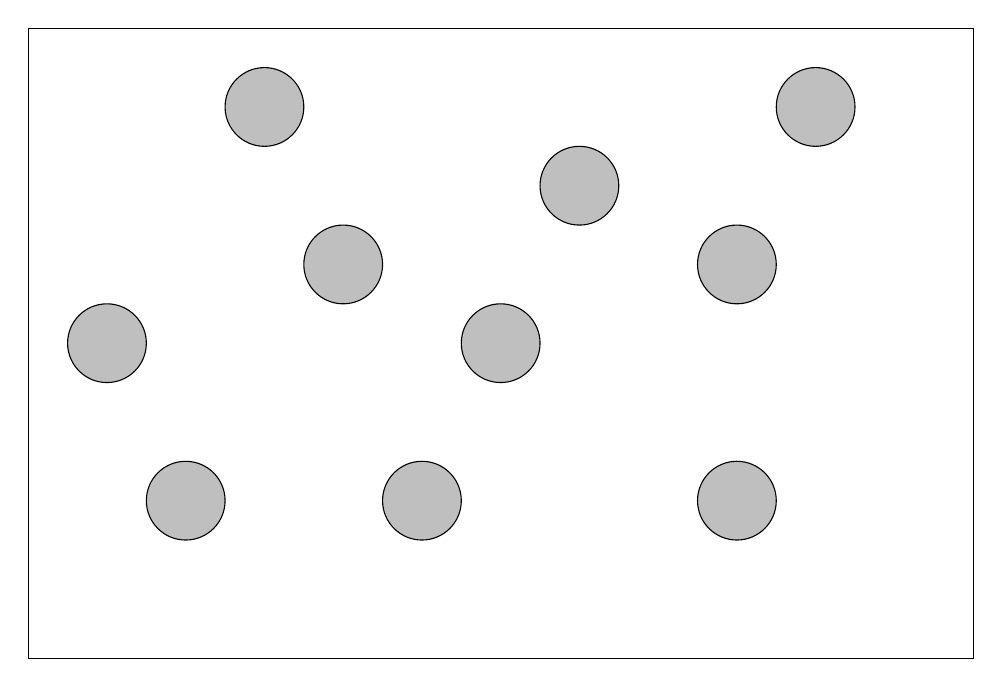
\begin{tikzpicture}

\draw[black] (0,0) -- (0,8) -- (12,8) -- (12,0) -- (0,0);
\filldraw[fill = lightgray, draw = black] (3,7) circle (0.5 cm);
\filldraw[fill = lightgray, draw = black] (1,4) circle (0.5 cm);
\filldraw[fill = lightgray, draw = black] (5,2) circle (0.5 cm);
\filldraw[fill = lightgray, draw = black] (6,4) circle (0.5 cm);
\filldraw[fill = lightgray, draw = black] (9,2) circle (0.5 cm);
\filldraw[fill = lightgray, draw = black] (2,2) circle (0.5 cm);
\filldraw[fill = lightgray, draw = black] (7,6) circle (0.5 cm);
\filldraw[fill = lightgray, draw = black] (4,5) circle (0.5 cm);
\filldraw[fill = lightgray, draw = black] (10,7) circle (0.5 cm);
\filldraw[fill = lightgray, draw = black] (9,5) circle (0.5 cm);
\end{tikzpicture}
\newline

Momentum is important because it describes how objects move in our Newtonian framework. We have written before that $\vec{F} = m\vec{a}$, but this is not quite correct. If you were like me, I am sure you wondered what would happen with force if the mass of the object was changing. Well, as you have probably assumed, it does not follow the fact that $\vec{F}=m\vec{a}$. Nature really follows the fact that \begin{equation}\vec{F}=\frac{d\vec{p}}{dt}\end{equation} Where $\vec{p}$ is momentum. For our purposes, we will define momentum relatively simply, $\vec{p}=m\vec{v}$. It is important to see here that momentum is our vector, just like velocity. This means that laws about momentum must hold in all of the three directions. It is easy to forget this because we will often only look at momentum in a single direction. Nonetheless, it is still important to understand its nature as a vector because more often than not, trick questions surrounding momentum in multiple directions will appear. Looking at momentum's of different objects will allow us to understand what happens during collisions. The examples we will describe may seem fairly contrived, but frankly, the world is made of collisions. Trillions of trillions of particles are hitting each other all the time. Think about air or water, or how any chemical reaction occurs. These things are the result of high-speed particles smashing into each other, sometimes heading their separate ways, and sometimes combining. We will see how to analyze these systems shortly. 

\subsection{Conservation of Momentum}
\begin{tikzpicture}
\draw[black] (0,0) circle (0.0001cm);
\draw[black] (3,0) circle (0.5cm);
\draw[black] (9,0) circle (0.5cm);
\draw[dashed] (3,-0.5) -- (5.75,-0.5) -- (5.75,-3);
\draw[dashed] (9,-0.5) -- (6.25,-0.5) -- (6.25,-3);
\draw (4.3,-0.25)node[anchor=west] {$V_{1x}$};
\draw (7.3,-0.25)node[anchor=west] {$V_{2x}$};
\draw (5,-1.5) node[anchor=west] {$V_{1y}$};
\draw (6.25,-1.5) node[anchor=west] {$V_{2y}$};
\draw (2.625,0) node[anchor=west] {$M_1$};
\draw (8.625,0) node[anchor=west] {$M_2$};
\draw[->] (3,-0.5) -- (5.75,-3);
\draw[black] (5.5,-3.25) node[anchor=west] {$v_1$};
\draw[black] (6,-3.25) node[anchor=west] {$v_2$};
\draw[->] (9,-0.5) -- (6.25,-3);
\end{tikzpicture}
\begin{center}
(Figure 5.2.1)
\end{center}
\
Now that we have introduced momentum we will describe collisions between two objects. Often these objects are described as square boxes but to make it more interesting and realistic; let us think of two gas particles colliding in the air around us. We will also assume that the two particles are so far away from any other particles, that they make up their isolated system. A few things can happen during collisions between particles, and they are all intuitive. The objects can collide and stay together, or they can collide and go separate ways. In the real world, we might additionally see a transfer of mass between the two particles but here, and for all AP Physics purposes, we will assume that this does not happen. So, we will now introduce the law of conservation of momentum. This law is pretty simple and is self-describing. The law says that the sum of the momentum of the particles before the collision is equal to the sum of the momentum of the particles after the collision,  assuming the system is isolated. This is identical to saying that the center of mass of the system has the same momentum before and after a collision. This law is not necessarily intuitive; in fact, I found it very hard to understand what this law was saying when I first learned about it. However, I feel that doing a few examples applying the concept can help build your intuition for it. First, let us assume that two objects of equal mass are moving directly towards each other with the same velocity. Let us assume that the objects are sticky and attach right after they collide. We assume that the collision happens extremely rapidly, so there is not an intermediate period during which the objects are not entirely connected. Here, we can essentially assume that the collision period is arbitrarily small. So what happens? Well, the objects will attach and switch the directions of their velocity but keep the magnitude of their velocity the same. Let us verify this using conservation of momentum.  So if we assign the axis on which the bodies are moving as the x-axis, the velocities of the bodies can be written as $v$ and $-v$. So if the bodies have the same mass, then the momentums of the bodies are $m\vec{v}$ and $-m\vec{v}$. So the total momentum in the x-direction before the collision was zero, and therefore the total collision after the collision is also. But if the two objects are attached, and the momentum of the system is zero, we can write \begin{equation}0=\vec{v}_{final} \left(m+M\right)\end{equation} Here we are treating the two-mass system as if it was a single mass but this is completely fine because they are attached, so they are essentially a single mass. From Eqn. 5.5.2, it should be fairly clear to see why the velocity of the two masses of the system after the collision was zero. Now let us do another example where the two objects stick together but where the colliding objects do not have the same masses and velocities. 

Let us assume that two objects of mass $m_1$ and $m_2$ are sliding in a frictionless plane with velocities $\vec{v}_1$ and $\vec{v}_2$ when they collide and attach. The momentum of the system before the collision was $m_1\vec{v}_1+m_2\vec{v}_2$ and it should stay that way until after the collision as well. But, the momentum of the system after the collision is \begin{equation}\vec{v}_{final}\left(m_1+m_2 \right)\end{equation} When we set these two expressions equal to each other we find that \begin{equation}\vec{v}_{final}=\frac{m_1\vec{v}_1+m_2\vec{v}_2}{\left(m_1+m_2\right)}\end{equation} This is a very elegant result, and we can look at some limiting cases to test if our expression is correct. First, let us assume that $m_1$ and $v_1$ are much greater than $m_2$ and $v_2$ respectively. This is essentially the scenario we have when a large bowling ball is coming by and hitting a ping pong ball is at rest. Let us assume somehow in our scenario that the hole of the bowling ball takes in the ping pong ball. Well in this case we have that  $$\vec{v_{final}} \approx \frac{m_1 v_1}{M_1}$$ Because $m_2\vec{v}_2$ and $m_2$ are negligible compared to $m_1\vec{v_1}$ and $m_1$ respectively. $\vec{v}_{final}$ is just $\vec{v}_1$ when simplifying. This should be intuitive. When a large object is coming faster hits and attaches itself to a tiny object at rest, the velocity essentially stays the same. What you may have noticed in these examples is that the kinetic energy of the objects does not stay constant. The kinetic energy has decreased in all of the examples we have seen. This may be especially disconcerting knowing that we have assumed there is no friction. Well, we have not violated the law of conservation of energy. Instead, the kinetic energy of the objects is lost to heat, sound, deformations, and many other things when the two objects collide. 

Another concern you may be having now surrounds objects under free fall. It appears as if the velocity of the ball is just rapidly increasing, which seems to be violating the law that momentum must be conserved. However, we have failed to take the whole system into account. In our model, we have looked only at the speed of the object changes. Indeed, if the ball were increasing in speed on its own, this would be impossible. However, the object does not make up its isolated system. Instead, the object is part of the earth-object system. So we have to take into account both the motion of the earth and the object to get the full picture of momentum. It turns out, when we do the calculations in later sections, that the sum of the momentum of the earth and the object during free fall stays constant. This may seem remarkable, but remember, this is just how nature is. 

When a collision occurs, and kinetic energy is conserved, we have what is called an elastic collision. When a collision occurs, and kinetic energy is not conserved, we have an inelastic collision. When we have a collision where the two bodies collide and stick together, this is a perfectly inelastic collision. It is called by this name because it entails the largest loss of kinetic energy possible while still obeying the conservation of momentum. We are now going to derive what happens in an elastic collision. In an elastic collision we have \begin{equation}m_1 v_1+m_2 v_2=m_1v_{a1}+m_2v_{a2}\end{equation} Where $\vec{v}_{1a}$ and $\vec{v}_{2a}$ are the velocities of $m_1$ and $m_2$ respectively after the collision. We have also assumed conservation of energy so \begin{equation}m_1\left(v_1\right)^2+m_2\left(v_2\right)^2=m_1\left(v_{a1}\right)^2+m_2\left(v_{a2}\right)^2\end{equation} I have gotten rid of the vectors here because when dealing with kinetic energy, we only have to think about the magnitudes of the velocities. I have also gotten rid of the factor of $\frac{1}{2}$ in front of each term because they cancel out. We will assume that $m_1$, $m_2$, $v_1$, and $v_2$ are known. So we have two equations in which there are two unknowns, $v_{a1}$ and $v_{a2}$. So, we should be able to solve this by substitution and using the quadratic formula. I will let you deal with these equations on their own as these formulas are used frequently, and useful insight can come from understanding them other than testing them at asymptotic cases. 

\subsection{Center of Mass}
\begin{tikzpicture}
\draw (0,0) -- (12,0);
\draw (3,0) -- (3,1) -- (9,1) -- (9,0);
\draw (3.25,1) -- (3.75,1.5);
\draw (4.25,1) -- (3.75,1.5);
\draw (3.75,1.5) -- (3.75,2.5);
\draw[->] (3.875,2) -- (4.5,2);
\draw (3.75,2.85) circle (0.35cm);
\end{tikzpicture}
\newline
The center of mass is an exquisite way to describe complex systems. Intuitively, the center of mass is the place where we can think all of the mass of the system as being located. Of course, this is not the case, but we can perform many calculations using this fact. The center of mass is a weighted average of the positions of the objects in a system with the weight being calculated with respect to the masses of the objects. Now we will see that we can think about conservation of momentum in terms of the conservation of momentum for the center of mass of a system. First, let us define the center of mass in one direction. \begin{equation}X_{CM}= \frac{\sum x_i m_i}{\sum m_i}\end{equation} The $x_i$’s here represent the positions of the masses in the systems, and the $m_i$’s are just the masses of the objects in the system. They can be negative depending on where we decide to make the position zero. Essentially, we sum the position of the object times its mass for each mass, and once we find that total sum, we divide the whole thing by the sum of all of the masses. So we can see that we have to multiply the position of the object times the mass of the object which gives more “weight” to the objects with greater mass. I was confused when I first encountered definition because it is not clear what the $x_i$ are. If we have two masses, who is to say which one is where? Well, we do not have to worry about this because the answer we will get will be the same no matter where we start. So, for example, let us imagine a system with two masses $m_1$ and $m_2$ separated by a distance $d$, and we are asked to find the center of mass of the system. This is quite an easy task. We just assume that $m_1$ or $m_2$ is at a position we call zero. Alternatively, we could assume that $m_2$ is at zero, or that the point directly in between them is zero. Ultimately, we will get the same answer. This is because the center of the mass will be relative to the point that we choose as 0. Let us do an example to clarify what I mean by this. So let us first say that $m_1$ is at zero. So the position of $m_1$ is zero and the position of $m_2$ is $d$, because $m_2$ is $d$ away from 0. We can therefore write that $$x_{cm} = \frac{m_2d+ m_10}{m_1+m+_2}$$ We simplify this to find that $$x_{cm} =\frac{m_2 d}{m_1+m_2}$$ this represents the center of mass as being $\frac{m_2 d}{m_1+m_2}$ away from $m_1$ in the direction of $m_2$. Now let us assume that $m_2$ is our zero point. $$x=\frac{0\cdot m_2+d\cdot m_1}{m_1+m_2}$$ You may now be thinking that we have gotten a different answer, but this is not, in fact, the case. This answer says that the center of mass is $\frac{dm_1}{m_1+m_2}$ away from $m_2$ in the direction of $m_1$. I challenge you to find the reason why these are the same answer. All it takes is some simple algebra and addition. Now, if you are still not convinced let us start from the point $\frac{d}{2}$ between the two objects exactly and that the x-axis goes from $m_1$ to $m_2$.  In this case \begin{equation}x=\frac{\frac{-d}{2}m_1+\frac{d}{2}m_2}{m_1+m_2}=d\frac{m_2-m_1}{m_1+m_2}\end{equation} Note that we have said the position of $m_1$ is negative because it is to the left of the middle between the two points and is therefore negative. This is once again the same answer. I challenge you to convince yourself of it using the same method you used above. There are some crazy things we can do using the center of mass. But first, we need to understand that the momentum of the center of mass will not change unless a force is acting upon the system. This makes sense because we can represent a whole system as just being the mass of the system at the point location of the center of mass. From this standpoint, we are just looking at how a mass will not change its momentum unless acted upon by an outside force. 

Let us do an example to make this more clear. We have a person on one side a box sliding along an ice court(assume an ice court is a frictionless plane). Our problem is to look at how much the box will move if the person will move to the other side of the box and there are no external forces. We assume the person has a mass $m_p$, the box has a mass $m_b$, and the length of the box is $l$. We can assume the person is so thin that they are exactly at the edge of the box. Initially, taking the middle of the boat to be the 0 point, the center of mass is \begin{equation}_{CM_1} = \frac{lm_p}{2\left(m_p+m_b\right)}\end{equation} After the person moves to the other side of the box, we can also calculate the center of mass as \begin{equation}X_{CM_2} = \frac{-lm_p}{2\left(m_p+m_b\right)}\end{equation} This result comes from taking the new location of the middle of the box as being 0. No external force was acting on the system so $$X_{CM_1}=X_{CM_2}$$ Therefore, for the center of mass to not change, the box must have moved $$\frac{lm_p}{m_p+m_b}$$ to the right.

Now that we have covered the example of the box on the frictionless plane, we should talk about another classic example: an astronaut floating away from their station in space with a tool in their hand. First, I want you to think for yourself about what happens when you throw something away from yourself back down on earth. Unless you are throwing something very quickly, nothing happens. This is because you and the ball are not an isolated system on earth. You are still being acted upon by a frictional force that acts against your motion. However, the frictional force is not there for an astronaut. So, using the same logic about the conservation of mass that we used for the boat example, we can reason about the motion of the astronaut. If the astronaut-tool system initially had no momentum and therefore a fixed center of mass, this will not change when the tool is thrown. So when the tool is thrown in one direction, the astronaut will go the other direction. This is quite useful for the astronaut, who would be floating away if he/she had not had the tool. 

The last thing we need to talk about is the fact that the center of mass can also be used if the system has an infinite number of masses. In this case, we can not rely on a simple formula, so we need to derive one that uses integrals to account for this type of situation. Fundamentally, the center of mass is the average location of mass within a system. That is all our formula was. Think about the ramifications of this and justify it to yourself with some simple examples. From calculus, we know that the average of a function over an interval is $$\frac{1}{length \ of \ interval}\int{f\left(x\right) dx}$$ For us, the interval we are looking at is all of the masses in the system. So the “length of the interval,” is just the sum of all of the masses in the system. Also, the $f\left(x\right)$ that we are averaging for is the position of each mass, and $dx$(represent each piece of the interval), is each piece of mass for us. So, if we write position as $r$, we get that \begin{equation}x=\frac{1}{M}\int{rdm}\end{equation} This formula may seem odd because we have never integrated over a mass before and we almost never do this integral directly. Normally, we will be given an expression for the mass density such as $\lambda=kr$. Where $k$ is a constant, $\lambda$ is the density of a small length of mass, and $r$ tells us how the density varies with a position at. I encourage you to do the example I have set up above with $\lambda=kr$ over a very thin stick(so thick that the stick is essentially a line). Imagine that the density at one end of the stick is 0 and at the other is $kl$, where $l$ is the length of the stick. This is a confusing topic, so do not worry if you get stuck. You only need to understand that $$dm=\lambda dr$$ and that ultimately, we are finding the average location of mass in the system. 

\pagebreak
\section{Circular and Rotational Motion}

\subsection{Angular Velocity and Acceleration}
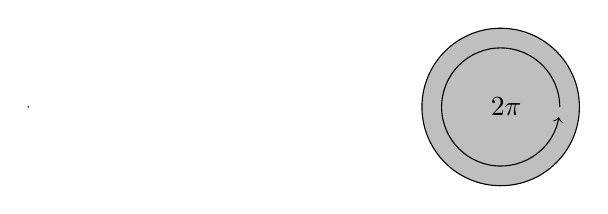
\begin{tikzpicture}
\draw (0,0) circle (0.0001cm);
\filldraw[draw = black, fill = lightgray] (6,0) circle (1cm);
\draw[->] (6.75,0) arc(0:350:0.75);
\draw (5.75,0) node[anchor=west] {$2\pi$};
\end{tikzpicture}
\newline

It can often be hard for people to learn about angular velocity because we see things spinning a lot less than we see them moving linearly. Up until now, we have only considered things moving around in space, but things can also spin. As we will see, there are many parallels between linear and rotational motion. The first thing we want to do is define angular velocity. Angular velocity will be a measure of how fast an object(perhaps a fidget spinner, or a disk), is rotating about a certain axis. Often the axis will be the center of the object, but it does not have to be. For our purposes, let us imagine that we have a disk rotating around its center, similar to how a fan spins. We can think about what happens during one time that it spins around. We say that in one revolution, the wheel would have spun around $360^o$. In radians, this corresponds to $2\pi$ radians. However, one weird thing about angular motion is that when an object has undergone a $2\pi$ radian movement, so it is essentially in the same position as before. If it went around again, we would say it has gone around $4\pi$ radians. This would not, however, be the case if we spun an object $2\pi$ radians clockwise, and then spun it counterclockwise. In that case, we would say the object had experienced a 0-radian angle change. So, essentially, even though either way the object looks the same before and after, we have a different change in the angle. This will be very important when talking about objects that might rotate thousands of times per second. However, we can also think about the rate at which the wheel is spinning. After all, a rotating disk will be of little use if it takes ten years before it can spin around one time. The rate at which a disk(or any rigid body for that matter), spins is called its angular velocity, $\omega$. A larger $\omega$ will correspond to the disk rotating around faster while a smaller $\omega$ corresponds to the disk rotating around more slowly. $\omega$ is defined as the number of radians that a point on a rigid body will move in one second. We can also define it in the same way as we defined linear velocity, as an angular displacement divided by a change in time. $$\frac{\Delta \theta}{\Delta t}$$ An angular displacement will be a slight change in the angle of the spinning object. So the object might turn a little bit. As you have probably seen plenty of times by now, we can take the limit of this equation to find that $$\frac{\Delta \theta}{\Delta t}$$ as $t$ goes to 0. We find that the instantaneous angular velocity is \begin{equation}\omega=\frac{d\theta}{dt}\end{equation} $\omega$ is called omega. This quantity will be in the units of radians per second. However, we do not consider radians in any practical matters(essentially we will pretend as if rads/second is just 1/seconds). Rigid bodies will have the same $\omega$ for all points on their surface by definition. This may seem odd, but you have to remember that angular velocity is only considered with rotation about an angle, and not necessarily about the true distance a point might be traveling. These definitions might have seemed kind of vague, but you will in time see that the idea is quite simple. Also, you will note that because $\omega$ is the same for all points on a rigid body, we will generally talk about the rotation of the whole body rather than the rotation of a specific point. 

Imagine we have a frisbee rotating about the top of my finger off of the center of the frisbee. Every $n$ seconds, the frisbee completes an entire rotation about the center of the frisbee. A rotation corresponds to an angular displacement of $2\pi$ radians. So the angular velocity is $$\frac{2\pi}{n} \frac{radians}{second}$$ using Eqn. 6.1.1. So moving every $\frac{2\pi}{n}$ radians takes 1 second for the frisbee to complete. Of course, closely related to the angular velocity is angular acceleration, which is much less intuitive but very important. Essentially, like acceleration, angular acceleration (symbolized by $\alpha$, pronounced alpha)  measures the change in angular velocity of a spinning object rather than a linearly moving object. It is defined as either $$\frac{d\omega}{dt}$$(for instantaneous acceleration), $$\frac{\Delta \omega}{\Delta t}$$(for average acceleration), or $$\frac{d^2\theta}{dt^2}$$ All three of these definitions can prove useful at the right times. Now, let us do a simple and contrived example to display angular acceleration. Say that an object is experiencing an angular velocity $\omega \left(t\right)$ that is changing as a function of time with $$\omega \left(t\right)=kt \frac{radians}{second}$$ We know that \begin{equation}\frac{d \omega}{dt}=\alpha\end{equation} so $\alpha=k$. This is a fairly boring question, a more interesting question might be, "by how many radians does the object rotate in time $t$?". To do this, we have to work from the angular velocity back to the angle by using integration, just like we did with linear velocity. We can say, as we did with the position, that the change in the angle of the object over a period is equal to the integral of the angular velocity of the object over the same time. So in our case the angular displacement is $$\int_{t_1}^{t_2} kt$$ is $$\frac{k\left(t_{2}^2-t_{1}^2\right)}{2}$$

\subsection{Constant Angular Acceleration}
\begin{tikzpicture}
\draw (0,0) circle (0.0001cm);
\filldraw (6,0) circle (0.05cm);
\draw (6, 0) -- (8, 1) -- (7, 3) -- (5, 2) -- (6,0);
\end{tikzpicture}

Now we are going to discuss perhaps the most boring topic that is covered in AP Physics C. That is, of course, constant angular acceleration problems. These problems are nearly identical to the linear constant acceleration problems so we will discuss these problems in brief and then talk about how we can relate the angular motion of the object and the linear motion of points on that object. First, we have the simplest relation which is that $\omega_0+\alpha t=\omega$, or equivalently, $\Delta \omega=\alpha t$. We also have that \begin{equation}\Delta \theta=\omega_0 t+\alpha \frac{t^2}{2}\end{equation} Or equivalently, \begin{equation}\Delta \theta=\omega_{final}t-\alpha \frac{t^2}{2}\end{equation} Additionally, we have that \begin{equation}\omega_{final}^2 = \omega_{0}^2+2\alpha \Delta \theta\end{equation} This is essentially the exact same formula as what we had with linear acceleration and we will be able to solve the problems the same way. 

It is necessary to discuss how we can relate linear and angular motion. We will first discuss this idea using the idea of a point on the edge of a frisbee. We can think about how much the point on the edge of the frisbee moves during one second to find the linear velocity of the point. The formula we find will be surprisingly simple. So if the frisbee rotates with a constant angular velocity $\omega$, then in $\frac{2\pi}{\omega}$ seconds, the object will have completed a complete revolution. This is because $$\Delta \theta=\omega \Delta t$$ If we plug in, we find that $$\Delta \theta=\omega \frac{radians}{s} \cdot \frac{2\pi}{\omega}s=2\pi \ radians$$ which corresponds to a complete revolution. So the period of the rotation of the frisbee is $\frac{2\pi}{\omega} \ seconds$. Now, we need to think about how much distance the point on the frisbee will travel during one rotation. We can assume the frisbee is circular so, during one rotation, the point should travel $2\pi r$ meters. Where $r$ is the radius of the frisbee. So if the object travels $2\pi r$ meters in $\frac{2\pi}{\omega}$ seconds, then the linear velocity of the object is $\omega r$ seconds. So we say that the linear velocity of the point is $v=\omega r$. In this case, $\omega$ is the angular velocity of the frisbee, and $r$ is the distance from the center of rotation to the point. This result hold for other objects that are not necessarily frisbees and for other points on the solid that are not necessarily on the edge of the surface. A good example might be a rectangle that is rotating about one of its corners with an angular velocity of $\omega r$ in the plane. This means that every $\frac{2\pi}{\omega}r$ seconds, the object will be in the same place that it was before and will have completed a complete rotation. We can say that the length of the rectangle is $l$ and the width is $w$. The angular velocity of the corner opposite to the one that is being rotated about is $\omega_r r$ where $r$ is the distance from the corner being rotated about to the opposite corner. Using the Pythagorean theorem, it is simple to see that $$r=\sqrt{l^2+w^2}$$ So the linear velocity of this point is $$\omega \sqrt{l^2+w^2}$$ Now, I only showed why in the case of constant angular velocity, even if the angular velocity is changing, $\omega_r r$ will still be equal to $v$. So if we have $\omega_r r=v$, we can differentiate both sides with respect to time and the two sides should still be equal because of $\omega_r r=v$ for all possible angular and linear velocities. However, if $\omega_r r=v$ were only true for this angular velocity, we would not be able to do this. So $\frac{dv}{dt}=a$ and $r$ is constant because the distance from the point we are recording to the center of rotation should not be changing with time. So $\omega_r r$ just equals $$r\frac{d\omega_r}{dt}=\alpha r$$ So the linear acceleration of a moving point on a rotating rigid body is the angular acceleration times the distance from the point to the center of rotation. This can, of course, be continued for further time derivatives but these will not be encountered, so we do not need to worry about them here. It is tough to have any intuition for these formulas, and they do not seem very applicable, but as we will see them later when discussing the rolling motion. 

\subsection{Angular Momentum}
\begin{tikzpicture}
\draw (0,0) circle(0.0001cm);
\filldraw (9,0) circle (0.25cm);
\draw[->] (8.75,0.3) -- (7.75,0.3);
\draw (8,0.5) node[anchor=west] {$\vec{v}$};
\draw (9.05,-1) node[anchor=west] {$\vec{r}$};
\draw (3,0) -- (9,0);
\draw[dashed] (9,-1.9) -- (9,0);
\filldraw (9,-2) circle (0.05cm);
\end{tikzpicture}
\newline
\newline
\newline
\begin{tikzpicture}
\draw (0,0) circle (0.0001cm);
\draw (3,0) -- (9,0);
\draw[->] (3,0) -- (3,1);
\filldraw (3,0) circle (0.05cm);
\filldraw (5,0) circle (0.05cm);
\filldraw (9,0) circle (0.05cm);
\filldraw (6,0) circle (0.05cm);
\draw (6,-0.25) node[anchor=west] {$X_{CM}$};
\draw (2.75,1.25) node[anchor=west] {$\vec{F_1}$};
\draw (4.75,0.75) node[anchor=west] {$\vec{F_2}$};
\draw (8.75,-2.25) node[anchor=west] {$\vec{F_3}$};
\draw[->] (9,0) -- (9,-2);
\draw[->] (5,0) -- (5,0.5);
\end{tikzpicture}
\newline
\newline
Angular momentum is \begin{equation}\vec{L} = \vec{r} \ \times \ \vec{p}\end{equation} This definition seems quite suspicious, and essentially, we only define it this way to make life convenient for us. Of course, we can see from this expression that it varies with how we define $r$. So we have to define the angular momentum of an object relative to a point in space. Frankly, this expression is tough to work with when we have a changing distance from the point to the object. So often times we will only use angular momentum when talking about circular and elliptical orbits. We can also see that if an object is traveling in a straight line relative to a point, the angular momentum will constantly be changing while the linear momentum is not changing. $\vec{p}$ here is the linear momentum of the object. The angular momentum $\vec{r} \times \vec{p}$ is a vector and will be perpendicular to the plane containing the position vector and the momentum of the object. The direction of this quantity is not physically meaningful, but its magnitude is very significant. We learned earlier that when no net force is being applied to an object, then the momentum of the object is constant. There is an analogy of this for rotational motion. When no net torque is being applied to an object relative to a point, the angular momentum of the object is constant relative to the point. We will define torque later, but for now, we will say that when the direction from the point to the object and the net force on the object are parallel, the torque on the object is 0. You can justify this to yourself through an example. If you have a rod with a nail in the midpoint that you can spin, if you try to pull the rod in the direction of the length of the rod, the rod will not spin. You can think about some simple applications of angular momentum where it is just plugging in, but we will discuss the real applications of it later when discussing gravitation. For now, let us imagine that an object is moving with linear velocity $\vec{v}$. Now find the angular momentum of the object relative to a point $d$ meters on top of the object. Assume the object starts moving at $t=0$, find the angular momentum at time $t$. We have that $$\vec{r}= \ \langle vt,d \rangle $$ and $$\vec{p}= \ <mv,0>$$ The magnitude of  $$\vec{r} \times \vec{p}$$ is equal to $$rp\sin\left(\theta \right)$$ where $\theta$ is the angle between $\vec{r}$ and $\vec{p}$. I encourage you to work out the cross product on your own. What you will find is that the angular momentum of the object relative to the point is equal to $$\langle 0,0,-dmv \rangle$$ regardless of the time which has elapsed. This should make sense because if no force is acting an the object, no net torque can act on it either, and therefore the angular momentum of the object must stay the same, nature works! This is exciting. I encourage you to come up with other fun examples of angular momentum as well, think about an object moving on the trajectory of a parabola. 

\subsection{Moment of Inertia}
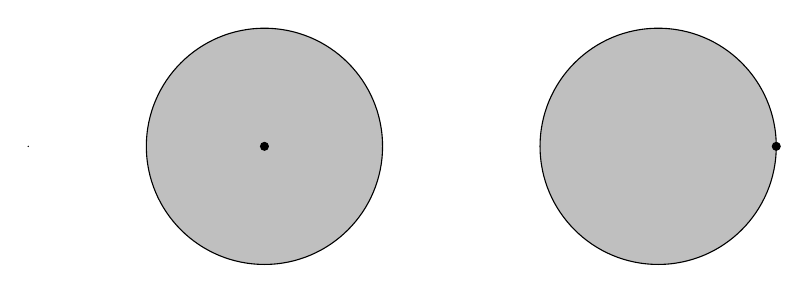
\begin{tikzpicture}
\draw (0,0) circle(0.00001cm);
\filldraw[fill = lightgray, draw = black] (3,0) circle (1.5cm);
\filldraw (3,0) circle (0.05cm);
\filldraw[fill = lightgray, draw = black] (8,0) circle (1.5cm);
\filldraw (9.5,0) circle (0.05cm);
\end{tikzpicture}
\newline

The concept of moment of inertia causes quite a good deal of trouble for many people because it is not something we can get an intuitive feel for and because it gets complex when we move beyond the most simple examples. However, if we clearly define the purpose of using the moment of inertia, it should make things much easier. Simply put, the moment of inertia is analogous to mass in linear motion. The larger the moment of inertia of an object, the “harder” it will be to accelerate it rotationally(and keep it going at a constant velocity when we have friction, as we will soon see, it will have units of $$kg \cdot m^2$$ Moments of Inertia are also confusing because their value is not only tied to the shape and size of the object, but also the axis around which the object in question is being rotated. To understand the need for the moment of inertia we first need to talk about angular momentum. Angular momentum is the momentum objects will have from rotating rather than from moving linearly. For a point mass, momentum $\vec{p}$ is equal to $m\vec{v}$. Angular momentum will be analogous to this. The analogy for $m$ will be I, and the analogy for velocity will be angular velocity, $\omega$. The symbol we normally use for angular momentum is $\vec{L}$ and in the right circumstances, is equal to $$I\omega$$ However, the true definition of the angular momentum of something about a point is $\vec{r} \times \vec{p}$. We assume that when we have rigid body motion, the object will be rotating about a certain point in circular fashion, so \begin{equation}\vec{r} \times \vec{p} = rp = mrv\end{equation} However, we have said that this is equal to $I\omega$. So we have that $$I\omega=mrv=mr^2\omega$$ so $I=mr^2$. This formula is only for a point mass rotating in a circle of radius r as part of a rigid body. It will not work when we have entire rigid bodies that are rotating. When we do this, we will talk about small masses, and tiny incremental moments of inertia, so we write that $dI=r^2 dm$. This is not anything new, but it will allow us to integrate over areas with changing radius or mass density to solve our problems. 

For example, let us first take the example of a perfectly flat frisbee(so we can ignore the third dimension) with surface density $\sigma$. This means that the mass of any region of the frisbee divided by that area is equal to $\sigma$. So, therefore the mass of the total frisbee is $$\pi r^2 \sigma$$ Now, we will use a sort of trick. We are to try to find the total moment of inertia of the frisbee by integrating over circles of different radii from 1 to r. We know that the mass of a circle of radius $r$ in general is $M=\sigma \pi r^2$. So, we can differentiate both sides of the equation with respect to r to find that \begin{equation}dM= 2\pi r \sigma dr\end{equation} This means that the mass of the little extra piece of a circle of radius $r+dr$ approaches $2\pi r \sigma dr$ as $dr$ goes to 0. I challenge you to find this yourself just using geometry. Well, we now have our expression for $dM$ as a function of the radius of the circle so we can integrate to find the moment of inertia. We have that $I= \int_{0}^{r} 2\pi r^3 \sigma \ dr$. We integrate from $0$ to $r$ because we are finding the mass of the little masses of circles from $0$ to $r$. When we integrate we find our expression is equal to $$\frac{\pi \sigma}{2} \cdot r^4$$ But $\sigma \pi r^2$ is equal to the mass of the frisbee, so the moment of inertia is $I = \frac{mr^2}{2}$. Now, this was a special example where we were rotating the frisbee about an axis parallel to its center of mass. However, often things will not rotate about their center of mass. It would be quite difficult to use our formula for the moment of inertia above when we are rotating about an axis not parallel to the center of mass. The integrals can get quite messy, and it is much easier to use the so-called parallel axis theorem. The parallel axis theorem states that the moment of inertia of a rigid body about an axis other than one parallel to the center of mass is equal to the moment of inertia about the center of mass, plus the mass of the object times the distance from the axis of rotation to the axis along the center of mass squared. In symbols, this is often written as \begin{equation}I=I_cm+mr^2\end{equation} I challenge you to use this formula to find the moment of inertia of a frisbee about its outer edge. Lastly, I challenge you to find the moments of inertia of a normal cylinder, a hollow cylinder, a sphere(this one is very tricky), and of a square about its center, a flat rod. You can assume you know both the mass of the item and the radius or length of it. We will see how important these are later, however, deriving them is mostly math and not physics, so they will not be covered here. In practice, you will often be able to look these up in a book. Lastly, it might be important for you to consider the moment of inertia of objects with holes. Although they do not appear on the AP Exam, the simple answer is that you can find the moment of inertia of objects with holes by imaging the hole wasn’t there and finding the moment of inertia, and then just finding the moment of inertia of what would be the mass of the hole, and then subtracting the second quantity from the first. Neat!

\subsection{Torque}
\
\
\
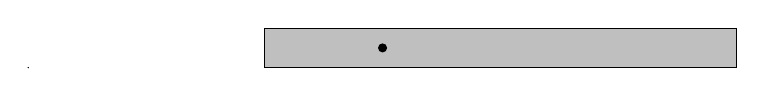
\begin{tikzpicture}
\draw (0,0) circle (0.00001cm);
\filldraw[fill = lightgray, draw = black] (3,0) -- (9,0) -- (9,0.5) -- (3,0.5) -- (3,0); 
\filldraw (4.5,0.25) circle (0.05cm);
\end{tikzpicture}
\newline
\newline
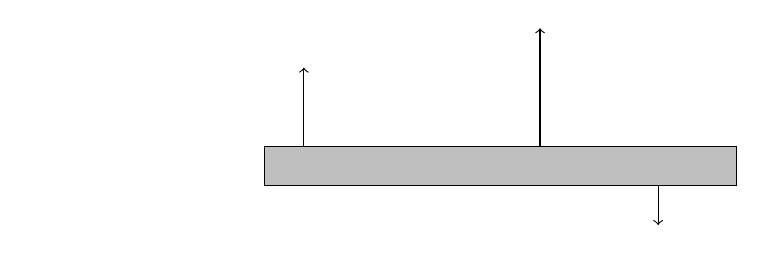
\begin{tikzpicture}
\draw (0,0) circle (0.000001cm);
\filldraw[fill = lightgray, draw = black] (3,0) -- (9,0) -- (9,0.5) -- (3,0.5) -- (3,0); 
\draw[->] (3.5,0.5) -- (3.5,1.5);
\draw[->] (6.5,0.5) -- (6.5,2);
\draw[->] (8,0) -- (8,-0.5);
\end{tikzpicture}
\newline
\newline
Torque is a relatively confusing topic because there are so few examples that we can see and relate it too. People move stuff and pick stuff up all the time, but very rarely do we rotate things at constant rates. Additionally, torque is a funny concept because it will vary with the point that we define it about. 

The first example can be the classic example of a rod pinned down at its end that we are trying to rotate around. We imagine that the axis of rotation is coming out of the page.  We know from our physical intuition that if we pull in the direction of the rod, the rot will not rotate, that would not make any sense. However, it is not necessarily clear that if we, for example, push a rod at a $45^o$ angle, that it will rotate any less fast than if we are to push a rod at a $90^o$ angle. However, tests have conclusively shown that the speed of acceleration of a rod given a certain pushing force, will vary with the $\sin$ of the angle between the force on the rod and the distance from the axis of rotation of the rod to the point where the force is being applied. It is also clear that if we are trying to rotate a rod, if we push directly at the point, or very near the point at which the object is being rotated, it will be tough to rotate the rod. It is not necessarily clear, however, that the farther along the rod that we push, the faster the rod will rotate given a certain constant force and angle of pushing against the rod. We can sum up these things that we see in nature in a relatively simple formula. This is that torque, denoted as \begin{equation}\vec{\tau}= \vec{r} \times \vec{F}\end{equation} Torque is the rotational analog of force, so we need to have a formula for torque analogous to $$\vec{F}=m\vec{a}$$ This is simple enough to create because $I$ is the rotational equivalent to $m$ and $\alpha$ is the rotational equivalent to $a$. So We have that $$\tau=I \alpha$$ Essentially this means that the torque being applied to an object is equal to its moment of inertia times the rate at which the object is accelerating angularly. Similar to angular momentum, we can see that torque is a vector, and its magnitude is equal to $$rp\sin\left(\theta \right)$$ where $\theta$ is the angle between the vector from the axis of rotation of the object and the direction of the force on the object. We can think about this with the example of two opposing forces operating on the same sides of a rod. It should be natural that if the forces are equal to each other, then the object will not rotate. We can verify this using the idea of torque and using the right-hand rule. Again, we can assume the object will rotate about its center so the $\vec{r}$ vector will be defined from the center of the rod to the edge of the rod, where the force is being applied. Torque is a difficult concept because often the axis of rotation may not be known, may be changing with time, or the force may be changing with time. This occurs when the object is not necessarily bolted to anything and maybe moving linearly in addition to rotationally, we will not see too many examples of this but as you might be able to tell, it can be tough to deal with these situations. 

\subsection{Angular Work and Power}
As we have seen with all of these other topics in angular mechanics, there is a clear connection between the angular and translation formulas. Angular work and power are no different. We think of angular work as being the work necessary to make an object spin for a certain period of time. Then angular power becomes the rate of work that is necessary to make the object spin at the rate that it is spinning it. Before we analyze any examples, let us find the correct formula for angular work. We know that the integral of force over a certain distance is equal to work so we can use our angular versions of force and distance to plug in and find our version of angular work. We find that the integral of torque over changes in the angle of rotation is equal to the angular version of work. Symbolically, that is \begin{equation}W_{angular} = \int \tau d\theta\end{equation}
We know that power is simply the time derivative of work so we can say that same thing for angular work. Lastly, we know that at a constant force, translational power is equal to $Fv$. We can replace both of these terms with their angular counterparts to find the angular versions of these formulas. We find that $P_{angular} = \tau \omega$

Now that we have these formulas down we will do some examples. 
First, let us find the power that must be delivered to a disk(assuming a perfectly flat disk) of mass M and radius R to allow it to rotate at an angular velocity omega w starting from rest in a time t. We know that the torque is equal to the moment of inertia of the disk times the angular acceleration of the disk. We will take the angular acceleration to be constant as the power being delivered to the disk is constant. We can use our equation for the angular velocity of an accelerating object $\omega_f=\omega_i+\alpha t$. Where $\alpha$ is the angular acceleration and $\omega$ is the angular speed. We assume that the initial angular velocity will be 0, so we have that $\frac{\omega_f}{t}$ is the angular acceleration. So $\alpha =\frac{\omega}{t}$. We also know that the moment of inertia for a flat disk is equal to $\frac{MR^2}{2}$. So we have the torque acting on the disk is equal to $\frac{M\omega R^2}{2t}$. We also know that from our formula for angular power, the power being delivered to the disk is equal to the torque times the angular velocity, so we find that \begin{equation}P = \frac{M\omega^2 R^2}{2t}\end{equation} Now, we need to check that this makes sense. First, it makes sense that if we can spend longer delivering power to the disk, we have to deliver less at each instant. Additionally, it would make sense that if we have a disk with a higher moment of inertia, that it is as if it was heavier and therefore would require more power to get it going at a certain speed. Lastly, it is obvious that if we want the disk to spin at a higher speed, assuming everything else is constant, we are going to have to deliver more power to the disk. We can use this formula for power to find out how much work it would take to accelerate the disk to the given angular velocity. We have to take the integral of the power with respect to time. However, before you begin integrating our expression with respect to time, it is essential to understand that our variable $t$ is the total time that it takes to accelerate our disk and not the time that has elapsed since we began accelerating the disk. If t were changing in time, then the power being delivered to the disk would not be constant, and this is not what we want. When we take the integral correctly, we find that the work that must be done to the disk is equal to $\frac{M\omega^2R^2}{2}$. This makes sense as it is just the rotational kinetic energy of the disk when it reaches the angular velocity w. Overall, angular work and power are relatively simple concepts once we understand their translational forms and the problems can mainly get harder if we assume a more complex system, but usually solving these requires more math than physics. For example, how much power does it take to get the water in a cup to move at angular velocity $v$ uniformly around the center of the cup in the horizontal plane? We can assume that the water is in the shape of a funnel, which we can model as a cone. An image is shown in Fig. 6.6.1.
\newline
\newline
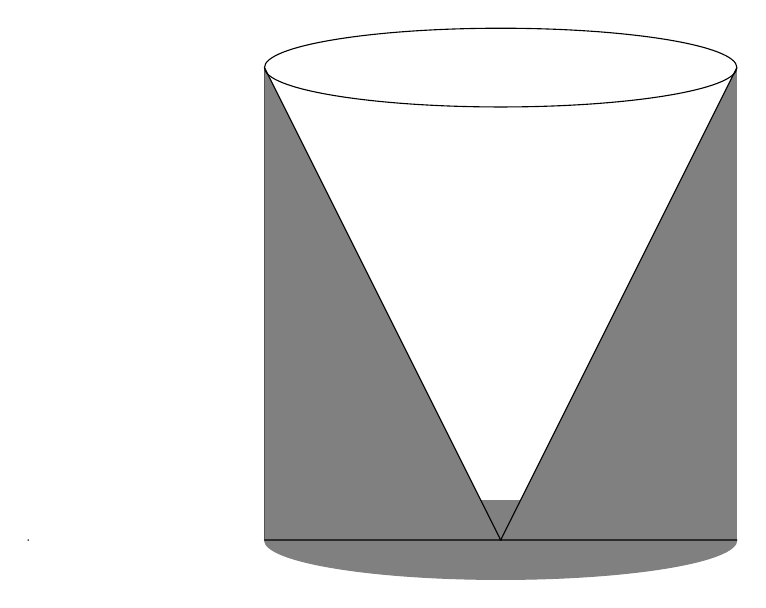
\begin{tikzpicture}
\draw (0,0) circle(0.0001cm);
\filldraw[fill = gray, draw=gray] (6,0) ellipse(3cm and 0.5 cm);
\draw (3,0) -- (3,6);
\draw (9,0) -- (9,6);
\filldraw[fill = gray, draw=black] (3,6) -- (6,0) -- (3,0);
\filldraw[fill = gray, draw=black] (9,6) -- (6,0) -- (9,0);
\draw (6,6) ellipse(3cm and 0.5 cm);
\end{tikzpicture}
\newline
\newline
\begin{center}
(Figure 6.6.1)
\end{center}
\subsection{Rotational Kinetic Energy} 
\  
\
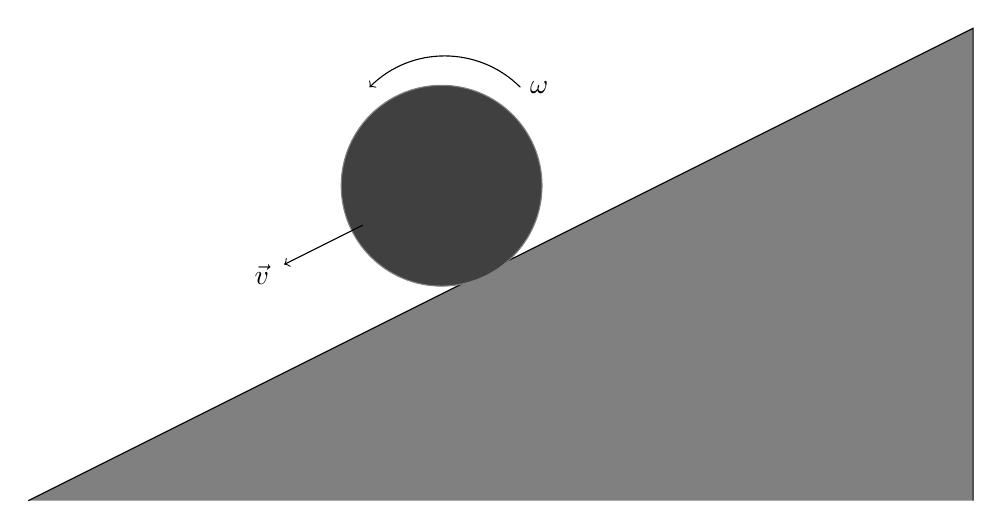
\begin{tikzpicture}
\filldraw[fill=gray, draw = black] (0,0) -- (12,6)--(12,0);
\filldraw[fill=darkgray, draw=gray] (5.25,4) circle (1.275cm);
\draw[->] (6.25,5.25) arc (45:135:1.355cm);
\draw (6.25,5.25) node[anchor=west] {$\omega$};
\draw[->] (4.25,3.5) -- (3.25,3);
\draw (2.75,2.875) node[anchor=west] {$\vec{v}$};
\end{tikzpicture}
\begin{center}
(Figure 6.7.1)
\end{center}
\
Rotational kinetic energy is the kinetic energy that objects get from spinning. The formula for rotational kinetic energy is akin to the formula for linear kinetic energy so I will just give it to you. \begin{equation}K_{rotational}=\frac{I\omega^2}{2}\end{equation} We can think of $I$ as being the mass and $\omega$ as being the velocity. This formula should match all of our intuitions. We will use it most often when considering objects that are rolling, that is, when objects are both rotating and moving linearly. In this case , when we want to use conservation of energy, we have to consider both the rotational kinetic energy and the linear kinetic energy, in some cases, we will just have to consider the rotational kinetic energy, if for example, a rotating disk is used to store energy in a car when it brakes and then power the car after. This is one reason why Tesla cars can be so efficient.

\section{Oscillations and Gravitation}
\subsection{Gravitation and Gravitational Potential Energy}
\
\
\
\
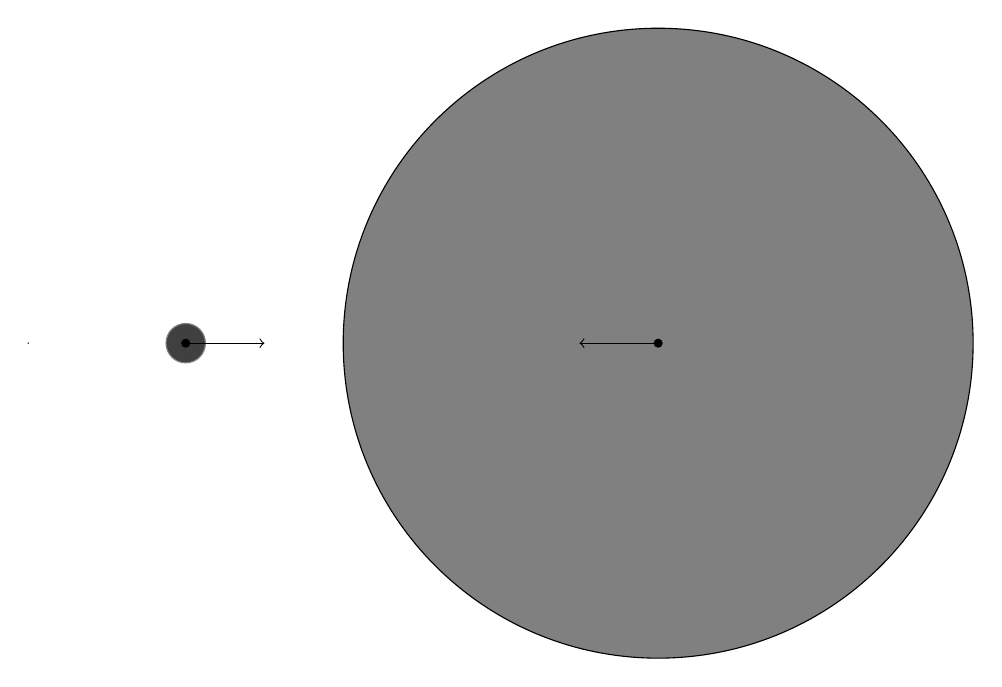
\begin{tikzpicture}
\draw (0,0) circle (0.0001cm);
\filldraw[fill = darkgray, draw= gray] (2,0) circle (0.25cm);
\filldraw[fill = gray, draw = black] (8,0) circle (4cm);
\filldraw (2,0) circle (0.05cm);
\filldraw (8,0) circle (0.05cm);
\draw[->] (2,0) -- (3,0);
\draw[->] (8,0) -- (7,0);
\end{tikzpicture}
\newline
Up until this point we have considered the gravitational potential energy as $mgh$ and the gravitational force as $mg$. However, this definition is only an approximation and only works in the case of an object of small mass that is very close to the surface of the earth. This should not be too much a surprise because it is not as if all objects in the universe are moving towards the earth with acceleration $g$. However, let us try to find out what the gravitational force is just using our intuition. Let us consider the case of two spheres of mass $m_1$ and $m_2$ in a vacuum separated by a distance $R$. It should be obvious that the gravitational force will increase if either one of the masses increases because there Will be more mass for the other mass to pull on. Additionally, it should be intuitive that the farther away the masses are, the smaller the gravitational force will be. We also should think that there will be some constant of proportionality between the factors that we have mentioned so far and the true factor. We will call this constant $G$. I am now going to assert because we can not show it analytically, that the gravitational force varies linearly with the two masses and varies as the inverse squared of the distance between the objects. So we can write that \begin{equation}F_g=\frac{-G m_1 m_2}{r^2}\end{equation} In one sense, we can say that we are now completely done with understanding Newtonian gravitation now that we have this expression. We can say this because we could model all items as being point masses and then plug in a vast number of atoms into our equations and use a computer to find how the atoms will behave. Doing work like this is very prevalent and important, and many numerical methods have been invented with the goal of trying to calculate the solutions to these problems. 
These types of problems quickly get very complicated. Think about it, with three masses; we have already a complex system where the force is constantly changing, and the objects are not going to behave in obvious ways.
\newline
\newline
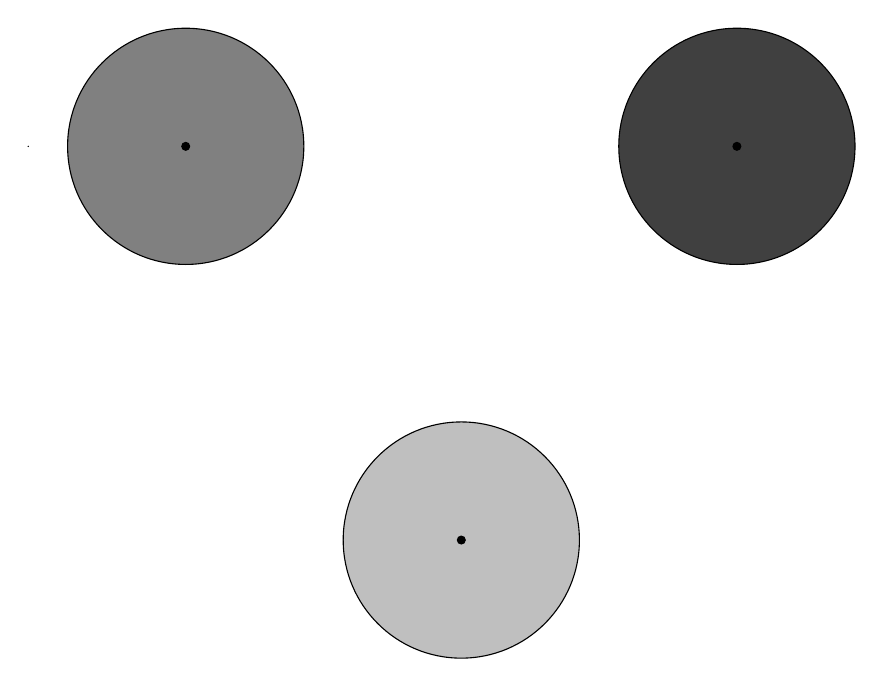
\begin{tikzpicture}
\draw (0,0) circle (0.00001cm);
\filldraw[draw = black, fill = gray] (2,0) circle (1.5cm);
\filldraw[draw = black, fill = darkgray] (9,0) circle (1.5cm);
\filldraw[draw = black, fill = lightgray] (5.5,-5) circle (1.5cm);
\filldraw (2,0) circle (0.05cm);
\filldraw (9,0) circle (0.05cm);
\filldraw (5.5,-5) circle (0.05cm);
\end{tikzpicture}
\begin{center}
(Figure 7.1.1)
\end{center}
\
Even if we use this formula to model an object falling to the earth, we already have to use numerical approximations. Most examples displaying this force will come in later sections, so, for now, we will move on to our discussion of the gravitational potential energy. 
To find the potential energy we are going to find the amount of work it would take to bring two objects from an infinite distance away to their current situation. At first, we imagine there is nothing where the masses are. Now we imagine moving the first mass in. This will not take any work as nothing is pushing or pulling on it to perturb it from its current state. So now we find the work it takes to bring the second mass from infinity to its current state, we will say at a distance $r$ from the other ball. This requires us to do an integral. I will leave this as an exercise to you, but upon completing the integral, we find that the potential energy \begin{equation} U = \frac{-Gm_1m_2}{r}\end{equation} This result is independent of which mass we imagine being brought in first as you can see when doing the calculation. We can use this concept of gravitational potential energy when discussing the motion of objects as they orbit around in space. 
\subsection{Gravitational Potential Energy and Satellites}
\
\
\
\begin{tikzpicture}
\draw (0,0) circle (0.0001cm);
\draw (11,0) arc (30:150:6cm);
\draw (5.5,3) -- (5.5,5);
\draw (6.5,3) -- (6.5,5);
\draw (5.5,5) --  (6,6) -- (6.5,5) -- (5.5,5);
\draw (5.5,3.5) -- (6.5,3.5);
\end{tikzpicture}
\begin{center}
(Figure 7.2.1)
\end{center}

We have already derived our formula for gravitational potential energy so now let us apply it to real situations. The first thing we can do is find the total energy of a satellite of mass m that is orbiting the earth at a radius $r$ from the surface. Due to a result that I will not prove known as Newton’s shell theorem, we can consider the gravitational effect of Earth to be the same as if all the mass of the object was concentrated at the center of mass of the Earth. This will work for any object and is a powerful result I challenge you to prove if you know multivariable calculus. 
We know that the gravitational potential energy is $\frac{-Gm m_e}{r}$. Now, we need to find the potential energy of the satellite. At first, it may not be clear how we are to find this as we have not been given the velocity, but I can calculate it using the fact the centripetal force in this problem is the gravitational force. Using this fact me can say that \begin{equation}\frac{mv^2}{r}=\frac{Gmm_e}{r^2}\end{equation} Therefore \begin{equation}K=\frac{mv^2}{2} = \frac{G m m_e}{2r}\end{equation} Adding this to the potential energy we find that the total energy of the satellite is equal to $$\frac{-G m m_e}{2r}$$ This means that the farther we go away from earth, the closer the potential energy goes to 0. At infinity, the total energy of the satellite will be 0. 
Using this fact, we can calculate the escape velocity of a ship from earth. This is the velocity that a ship, or any other object for the matter, will need to escape from earth. This may seem complicated, but all we have to do is set the energy that the ship has at the surface equal to the energy that the satellite has at infinity. So we find that \begin{equation}0=\frac{-G m m_e}{r_e}+\frac{mv_{e}^2}{2}\end{equation} where $r_e$ is the radius of the earth. Solving this equation for $v_e$, we find that $$v_e=\sqrt{\frac{2Gme}{r_e}}$$ It is important to understand that even though we call this the escape velocity, a ship does not have to go exactly this speed to be able to escape the gravitational pull of the earth. This is simply the minimum velocity necessary to prevent the object from orbiting around the earth. 
Now let us think about an object that is orbiting the earth at a radius $r_1$ and something happens and its radius of orbit suddenly changes to $r_2$. We want to find by how much the speed of the object changed. We know that the kinetic energy of the object is equal to $\frac{G m m_e}{2r}$. So, we can solve for the velocity of the object in terms of the radius at which it is orbiting. We find that the velocity is equal to $$\sqrt{\frac{Gmme}{r}}$$ So if the the radius changes from $r_1$ to $r_2$, the velocity changes by $$\sqrt{\frac{G m m_e}{r^2}}-\sqrt{\frac{G m m_e}{r1}}$$ So, if $r_2$ is greater than $r_1$, the velocity has decreased and if $r_2$ is less than $r_1$, the velocity must have increased. This means that the closer the object is to earth, the faster it is orbiting around the earth.
One thing you might have been thinking is that because of Newton’s third law, the Earth will attract an object orbiting around it, but the object must also attract Earth! This is completely correct. An object orbiting around another object is not orbiting just around the object, it is orbiting around the center of mass of the object-object system. This center of mass is called the barycenter. For a system with the earth and an object of small mass, the center of mass is so close to the center of Earth that any deviation is negligible. However, for star-star systems, this difference is significant. Calculating orbits in these systems can be very complicated, so I will not show you any examples here.
\subsection{Kepler's Laws}
\
\
\
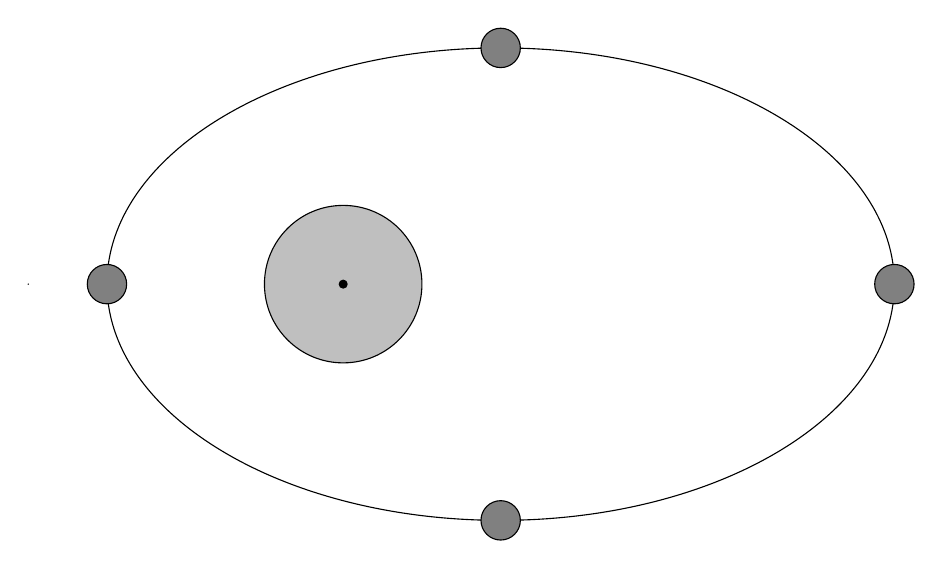
\begin{tikzpicture}
\draw (0,0) circle (0.00001cm);
\filldraw[fill = lightgray, draw = black] (4,0) circle (1cm);
\filldraw (4,0) circle (0.05cm);
\draw (6,0) ellipse (5cm and 3 cm);
\filldraw[fill = gray, draw = black] (1,0) circle (0.25cm);
\filldraw[fill = gray, draw = black] (11,0) circle (0.25cm);
\filldraw[fill = gray, draw = black] (6,3) circle (0.25cm);
\filldraw[fill = gray, draw = black] (6,-3) circle (0.25cm);
\end{tikzpicture}
\begin{center}
(Figure 7.3.1)
\end{center}
\
Kepler’s Laws of gravitation truly are not that special and are mainly taught for historical reasons. They can be derived from Newton’s Laws alone. Nonetheless, they are very interesting.

The first law is a proclamation that planets orbit the sun in elliptical orbits with the sun at one focus of the ellipse. If you are not sure about the definition of an ellipse, I recommend you read up about conic slices as they turn out to be quite crucial in describing the orbits of planets. This is not entirely true because Newton’s Laws are not a complete description of gravity. The planets orbit the sun in a sort of helix that when you view from above, appears to make an elliptical orbit. From year to year this transition may be minimal, but over a long time, this effect becomes significant. I will not present the proof of this, but I do recommend you look at a 3Blue1Brown video on his youtube channel and on the minutephysics channel where they talk about this topic. 

The second of Kepler’s Laws tells that if you draw a line from a planet orbiting the sun to the sun and calculate the area that this line sweeps out in a time t, that this area will be the same regardless of the part of the orbit that the planet is in. Graphically, this is represented in Fig. 7.3.1. I will not attempt to prove this to you either because it requires some more sophisticated mathematics but the physical principle used to prove this involves the conservation of angular momentum. 

The last of Kepler’s Laws we will prove in a special case. The third law states that the square of the period for a planet orbiting a star is proportional to the third power of the length of the semi-major axis of the elliptical orbit. For the case of a circular orbit, the length of the semi-major axis is simply the radius of the orbit. So we can use the concepts we have learned so far to prove this true in the special case. We can say that $$\frac{m_1v^2}{r} =\frac{Gm_1m_2}{r^2}$$ $m_1$ here is the mass of the planet and $m_2$ is the mass of the sun. $v$ is equal to the circumference of the circle divided by the period of the circle. \begin{equation}v=\frac{2\pi r}{T}\end{equation} So \begin{equation}\frac{4 \pi^2 m_1 r^2}{T^2}=\frac{Gm_1m_2}{r^2}\end{equation} We finally have that \begin{equation}T^2=r^3 \left(\frac{4\pi^2}{Gm_2}\right)\end{equation} This is the result that we wanted.
\subsection{Simple Harmonic Motion}
\
\ 
\newline
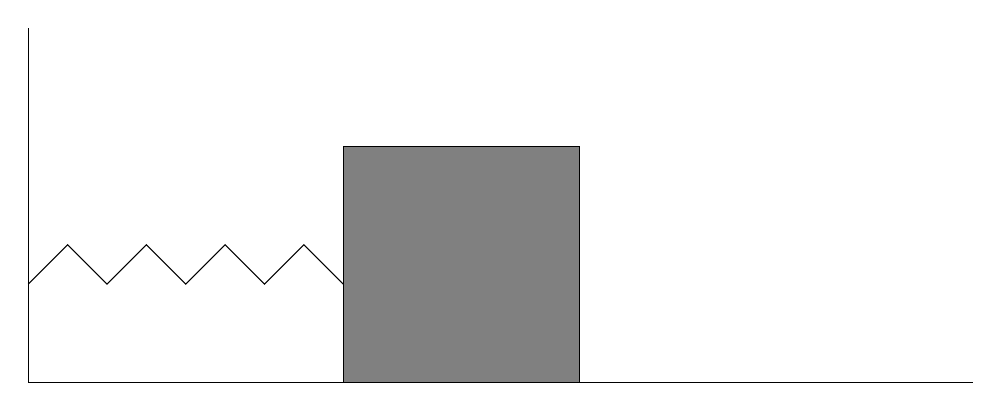
\begin{tikzpicture}
\draw (0,0) -- (12,0);
\draw (0,4.5) -- (0,0);
\filldraw[fill=gray] (4,3) -- (4,0) -- (7,0) -- (7,3) -- (4,3);
\draw (4,1.25) -- (3.5,1.75) -- (3,1.25) -- (2.5,1.75) -- (2,1.25) -- (1.5,1.75) -- (1, 1.25) -- (0.5,1.75) -- (0,1.25);
\end{tikzpicture}
\begin{center}
(Figure 7.4.1)
\end{center}
\
We will now begin discussing something that occurs very frequently not only in elementary physics but in more advanced physics. Often complex systems can be modeled using a system of simple harmonic systems. For example, we can model atom-atom interactions in solids as being a giant set of balls with strings attached between them approximating the force between the atoms. However, before we get there, we will consider the simple case of a spring pushing a mass m along a frictionless table as seen in Fig. 7.4.1. 


In these problems, we almost always take the approximation that the spring is massless. We can define a point called equilibrium at which, if not perturbed, the spring will not contract or expand. We can also assume that the spring enacts a linear restoring force upon the mass. This means that the force that the spring enacts is either pushing or pulling to the mass is proportional to the distance the mass is from equilibrium. We call the distance that the mass is away from equilibrium $x$ and we call the constant of proportionality between the distance and the true force $k$. It is important to recognize that the factor $k$ depends not on the mass, but on the spring itself. A more stiff string will be less happy to tolerate deviations away from its natural length, and therefore the restoring force will be greater. Meanwhile, a less stiff string will be more happy with deviations, and the restoring force will decrease. Because $k$ is proportional to the restoring force, it must be greater for more stiff strings and smaller for less stiff strings. 
We now know the magnitude of the restoring force, but we need to think of its direction. If you think about extending a string beyond its natural length while keeping one end fixed, there is going to be a force in the direction opposite to the direction of extension. Likewise, if we contract the spring, there is going to be a force in the direction opposite to how we contracted the spring. For this reason, we take the restoring force $F_{elastic}$ to be equal to $-kx$. Armed with this formula, we can use Newton’s second law to find the equation of motion for a mass $M$ that is moving with a string. We imagine that the string was displaced from the equilibrium at a distance $A$, where $A$ is the amplitude. We write that $ma=-kx$ as no other forces are involved in describing the motion of the system. We note that if $x=0$, then the acceleration is 0 and the system should not move. Simply moving the -$kx$ term to the other side and dividing both sides my m we find that \begin{equation}a+x\left(\frac{k}{m}\right)=0\end{equation}
We note that $a$ is just the second time derivative of $x$. We notice that because $k$ and $m$ are both positive, $a$ and $x$ must be of the reverse sign. Additionally, $a$ has to be equal to a constant multiple of $x$. Using these facts we can think about a function of $x$ with respect to $t$ that might satisfy these constraints. A polynomial won’t work because the second derivative of a polynomial is not a constant multiple of the original polynomial. Neither will an exponential because the second derivative of an exponential will be of the same sign as the original polynomial. However, a trigonometric function will work. The second derivative of $$a\cos\left(kx\right)$$ with respect to $x$ is simply $$-ak^2\cos\left(kx\right)$$ So if we take $x$ to be equal to $$A\cos\left(\omega t \right)$$ we find that $$-A\omega^2\cos\left(\omega t \right)+A\left(\frac{k}{m}\right)\cos\left(\omega t \right)=0$$ If we solve this equation, we find that $\omega$ is equal to $$\sqrt{\frac{k}{m}}$$ So our expression for $x$ is currently $$A\cos\left(\sqrt{\frac{k}{m}}t\right)$$ We assumed that at $t = 0$, and that the mass was displaced from equilibrium by a distance equal to the amplitude, so $x\left(0\right)$ must be equal to $A$. So in our expression, $A$ is the amplitude of oscillation. One thing we notice is that $x$ can never be greater than $A$ or less than $-A$ because a cosine function never is greater than 1 or less than -1. We can also note that the period of oscillation is equal to $$\frac{2\pi}{\omega}$$ The period of oscillation is the time it takes the spring to get back to the point where it originally was after leaving that point. This is just a general property of trigonometric functions that is best for you to discover on your own.  The frequency of oscillations is one divided by the period and is simply the number of complete oscillations that the system completes every 1 second. If you are not convinced, I challenge you to think a bit more about this point as it can be confusing at first. 
Now that we have derived the equation of motion for a horizontally moving mass and spring system, I challenge you to do the same thing for a similar system that is oscillating vertically. You can make a similar equation to the differential equation I have made before and attempt to solve it, but this will prove very difficult unless you have taken a course in differential equations. However, what you can do is imagine that the equilibrium is at the point at which the gravitational force acting on the mass is equal to the spring force acting on the box. We can take this point as being equal to 0, and then we have a normal mass-spring system. I challenge you to work out the specifics using both methods to see why the second one is much preferable.  

We have worked out the equation of motion for this string using Newton’s laws, but as we saw with other problems in Newtonian dynamics, we can formulate this problem in terms of energy. We will say that the potential energy of the system plus the kinetic energy of the system is constant because no work is being done on the system.  We will analyze the same system as above. The kinetic energy of the system is equal to $\frac{mv^2}{2}$ where $v$ is the velocity of the mass. The potential energy we can find by integrating the force that the spring does on the mass. Upon integrating, we find that the potential energy of the spring is equal to $\frac{-kx^2}{2}$, where $x$ is the distance displaced from equilibrium. With these two terms, we find that $$\frac{mv^2}{2}+\frac{kx^2}{2}$$ is a constant. This means that when one term is at the maximum, the other must be at a minimum. We can also find this by using the equation of motion in terms of sines and cosines we found above. The velocity will be 0 when the distance displaced is highest and vice versa. If you are not convinced by my work, I recommend you watch a good Walter Lewin video where he describes this topic. He also shows some demos that may help convince you that simple harmonic oscillation can be described using just sines and cosines. 

\subsection{Pendulums}
\
\
\
\begin{tikzpicture}
\draw (0,0) circle (0.00001cm);
\filldraw (6,0) circle (0.05cm);
\draw (7,-2) -- (6,-0);
\draw[->] (8,-4) -- (7,-2);
\filldraw (8,-4) circle (0.5cm);
\draw[->] (8,-4.5) -- (8,-5.5);
\draw (8,-5.5) node[anchor=west] {$\vec{F_g}$};
\draw (7,-2) node[anchor=west] {$\vec{F_T}$};
\draw[dashed] (7.625,-4.375) arc (-45:-135:3cm);
\end{tikzpicture}
\begin{center}
(Figure 7.5.1)
\end{center}
\ 
\
Now, we will talk about pendulums, one of the few other examples of simple harmonic oscillation that we will see in elementary physics. We will consider a pendulum with length $L$ of negligible mass with a small ball of mass $M$ attached to its bottom. We take the size of the ball to be negligible compared to the length of the pendulum. We assume that the pendulum is fixed at its top. 
The pendulum moves along a curve where its velocity will always be perpendicular to the string. This means that the tangential velocity of the ball is perpendicular to the string, and therefore the tension force. Therefore, when we are considering moving in the tangential direction, we do not have to worry about the tension force. We can not think about this as a normal centripetal acceleration problem with the tensional force as the centripetal force because the velocity of the ball is constantly changing due to gravity. So, now let us think about the forces acting on the ball in the tangential direction. We see that the only force in this direction is the gravitational force. The gravitational force in this direction is equal to $$mg\sin\left(\theta \right)$$ We will take the approximation for small angles that $\sin\left(\theta \right)$ is simply equal to $\theta$. We take this approximation simply because it is too difficult to solve the differential equation that results from this expression if we do not. This approximation is so common that it gets the name the small angle approximation. If this doesn't seem obvious to you, I recommend you to work this out on your own because situations like this occur very frequently. We can now write that $$-mg\theta=mat$$ We added the - sign because the force is a restoring force(in fact it is a linear restoring force in $\theta$). We can also say that $L\alpha=at$ because the pendulum is a rigid body that is undergoing angular acceleration. We note that $\alpha$ is the second derivative of theta. We can cancel the $m$’s and move the $g\theta$ term to the other side followed by dividing by $L$ to find that \begin{equation}\alpha+\theta \left(\frac{g}{L}\right) =0\end{equation} This is exactly what we had in the normal situation for harmonic oscillation. We can take $\omega^2$ to be $\frac{g}{L}$. Using this we can determine the period of oscillation for the pendulum in addition to the frequency of the system. The period is equal to $\frac{2\pi}{\omega}$ and therefore $$2\pi \sqrt{\frac{L}{g}}$$ This makes sense. We would imagine a longer string would take longer to make a complete oscillation, and we would imagine if $g$ was greater, and the force of gravity was, therefore, greater, that the period of oscillation would decrease. Using what he has done so far, I leave it to you as an exercise to calculate the frequency of the pendulum and for more of a challenge, calculate the frequency and period where we take an arbitrary object to the pendulum. You will have to use torque and the center of mass in addition to the small-angle approximation to find your answer. However, in theory, it is not that difficult to do. Hopefully, you have seen through this example how powerful an approximation can truly be. 
\pagebreak
\section{Conclusion}
Now that you have completed the book I hope that you are prepared for the Physics C: Mechanics exam. I also hope that you can better appreciate the joy of physics and understand the subtleties of the subject. I hope you will be encouraged to learn more. We have learned a lot of interesting things, but of course, there is so much more that we can do. There is a lot left for you(and for me), to learn. Thank you for taking the time to read the book, and I wish you well.
\newline
-Leo

\end{document}